\chapter{Corriente alterna}

Cuando en una gráfica de \textbf{tensión en función del tiempo} se observa un nivel de tensión por arriba del eje de abscisas, se considera positivo. Cuando está por debajo del eje, se considera negativo, y por lo tanto, representa a una corriente que está circulando en sentido contrario.
 
De esa manera, una tensión que se encuentre sin cruzar el eje en un determinado período de tiempo, se denomina \textbf{continua}. Si el sentido de la corriente cambia de forma periódica (es decir, pasa de negativa a positiva o viceversa, y se repite su forma de onda al transcurrir un determinado tiempo), se denomina \textbf{alterna}.
\begin{ejemplo}
	En las imágenes se pueden apreciar distintas variaciones de la tensión a lo largo del tiempo.
	\begin{itemize}
		\item En la \textbf{figura \ref{fig:acdc_a}}, la tensión es continua.
		\item En la \textbf{figura \ref{fig:acdc_b}}, la tensión es alterna, y tiene una forma de onda cuadrada.
		\item En la \textbf{figura \ref{fig:acdc_c}}, la tensión es alterna, y tiene una forma de onda senoidal.
		\item En la \textbf{figura \ref{fig:acdc_d}}, la tensión, si bien tiene forma de onda senoidal, es continua, porque se encuentra siempre por arriba del eje de abscisas. En otras palabras: nunca cambia su sentido, sino que sólo varía su valor de tensión.
	\end{itemize}
\end{ejemplo}

\begin{figure}[htbp]
  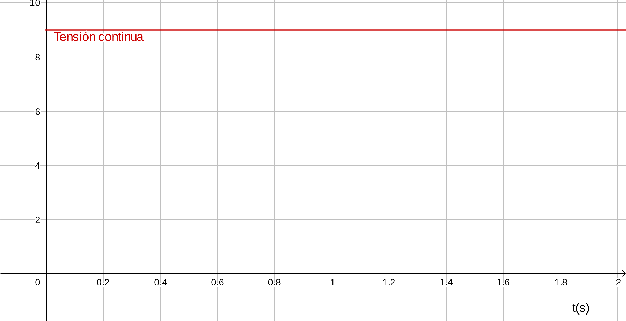
\includegraphics[scale=0.75]{images/acdc_a}
  \caption{Corriente continua}
  \label{fig:acdc_a}
\end{figure}
\begin{figure}[htbp]
  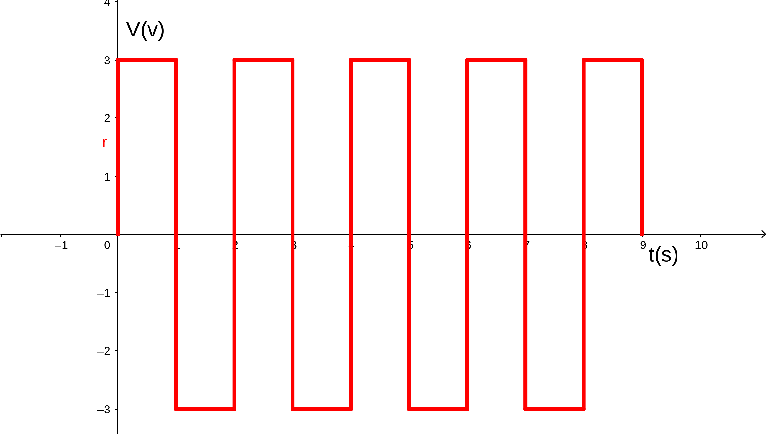
\includegraphics[scale=0.6]{images/acdc_b}
  \caption{Corriente alterna cuadrada}
  \label{fig:acdc_b}
\end{figure}
\begin{figure}[htbp]
  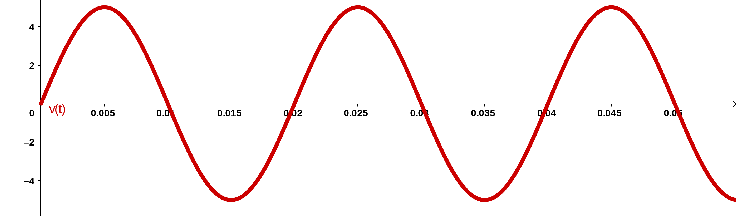
\includegraphics[scale=0.14]{images/acdc_c}
  \caption{Corriente alterna senoidal}
  \label{fig:acdc_c}
\end{figure}
\begin{figure}[htbp]
  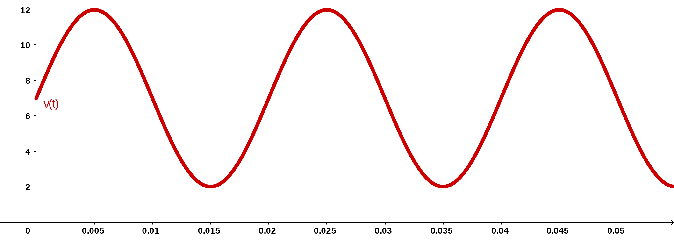
\includegraphics[scale=0.6]{images/acdc_d}
  \caption{Corriente con forma senoidal no alterna}
  \label{fig:acdc_d}
\end{figure}
Si bien existen varias formas de ondas de corriente alterna (triangular, cuadrada), la más difundida es la \textbf{forma senoidal}, que se puede apreciar en la figura \ref{fig:acdc_c}. Esto es así, porque es el voltaje que se genera en las plantas eléctricas y porque, además, permite realizar ciertos cálculos matemáticos que la explican y predicen, aunque son algo más complejos que los de corriente directa o continua.

\section{Corriente alterna senoidal}

En la figura \ref{fig:ac} se puede distinguir una onda alterna senoidal. Pueden distinguirse los siguientes parámetros:

\begin{itemize}
	\item Valor instantáneo: magnitud de una forma de onda en cualquier instante. Se han indicado como ejemplos $e_1$, $e_2$ y $e_3$.
	\item Valor pico: valor instantáneo máximo medido con respecto al nivel de 0 Volts. En la gráfica, se indicó como $Vp$. También se indicó el valor de pico negativo como $-Vp$.
	\item Valor pico a pico: tensión entre $Vp$ y $-Vp$. Es la suma entre las magnitudes de los valores de pico positivo y negativo.
	\item Ciclo: parte más pequeña de una onda hasta que comienza a repetirse.	
	\item Periodo $T$: Tiempo que dura un ciclo. En el ejemplo se tiene 3 periodos (de $O$ a $T_1$, de $T_1$ a $T_2$ y de $T_2$ a $T_3$, aunque pueden indicarse otros periodos).
	\item Frecuencia $f$: es la cantidad de ciclos que ocurren en 1 segundo. La frecuencia se mide en hertz (Hz), donde $1\; Hertz = 1\; \text{ciclo por segundo}$.
\end{itemize}

Del desarrollo anterior, se desprende que:
\begin{equation}
	\label{eq:frec_ciclos}
	f=\frac{1}{T}
\end{equation}
Y que:
\begin{equation}
	\label{eq:ciclos_frec}
	T=\frac{1}{f}
\end{equation}
Donde \textbf{T} se mide en segundos, y \textbf{$f$} se mide en Hz (Hertz).
\begin{figure}[htbp]
  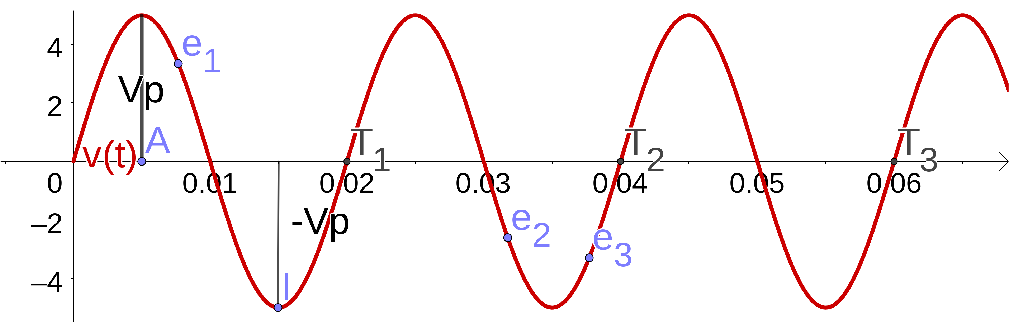
\includegraphics[scale=0.14]{images/ac}
  \caption{Corriente alterna senoidal: parámetros}
  \label{fig:ac}
\end{figure}
\begin{ejemplo}
	\label{ej:ac_argentina}
	En la figura \ref{fig:ac_argentina} se puede apreciar una onda senoidal que representa la tensión utilizada en Argentina.
	
	El valor de pico es $Vp = 311\; V$ y el periodo $T = 0,02\; s$.
	
	La frecuencia es $$f=\frac{1}{0,02\; s}=50\; Hz$$
	
	El valor de pico a pico es $$ Vpp = 2 \times 311\; V = 622\; V $$
\end{ejemplo}
\begin{figure}[htbp]
  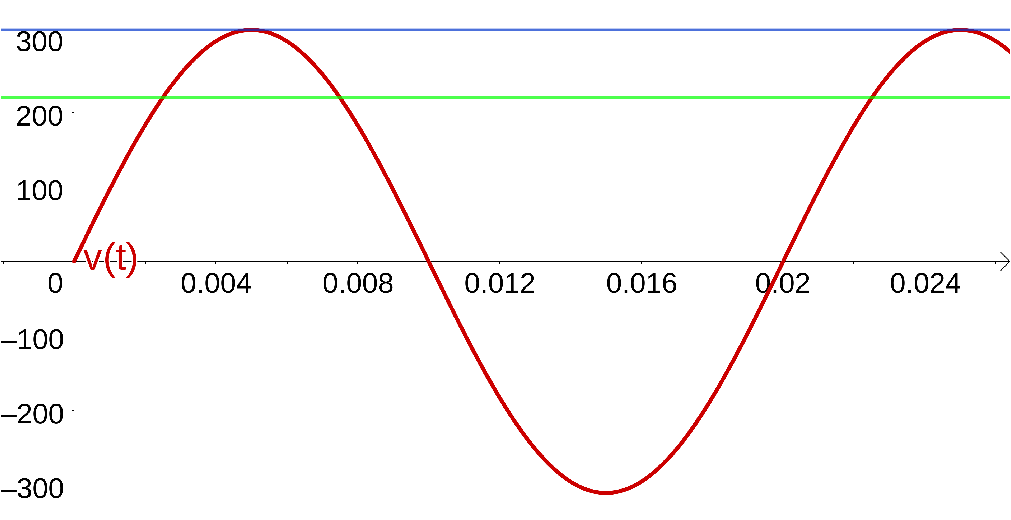
\includegraphics[scale=0.1]{images/ac_argentina}
  \caption{Corriente alterna en Argentina. En color azul, la tensión de pico y en color verde, la tensión eficaz}
  \label{fig:ac_argentina}
\end{figure}

\subsection{Definición matemática}
Si se desea considerar a la tensión (en voltios) en función del tiempo (en segundos) para una forma de onda senoidal, se deberá partir de la función $$v(\alpha) = sen (\alpha) $$
Obsérvese que en vez de utilizarse la variable $t$ (que se suele utilizar para indicar tiempo como número real), se ha definido un ángulo $\alpha$. Esto se debe a que la función senoidal está definida como el conjunto de valores que se obtienen al proyectar verticalmente un vector de radio que gira con movimiento circular uniforme alrededor de un punto fijo. La forma senoidal completa se trazará luego de haber completado una rotación de 360 grados alrededor del centro (o $2\pi$ radianes).

Suele ser más cómodo trabajar con \textbf{radianes} en vez de \textbf{grados sexagesimales} para medir los ángulos y es lo que se hará en este texto.

La idea de \textbf{proyectar verticalmente} el vector proviene de la trigonometría, ya que el $sen \alpha = \frac{\text{cateto opuesto}}{\text{radio}}$, como puede apreciarse en la figura \ref{fig:seno_triangulo}. Como el radio del vector es 1, entonces $ sen \alpha = \text{cateto opuesto} $, que es la \textbf{proyección vertical} del vector.

\begin{figure}[htbp]
  \includegraphics[scale=0.1]{images/seno_triangulo}
  \caption{Seno en un triángulo rectángulo}
  \label{fig:seno_triangulo}
\end{figure}

Un desarrollo de esta idea puede apreciarse en la figura \ref{fig:seno_proyectado}.
\begin{figure}[htbp]
%  \includegraphics[scale=1]{}
  \caption{Forma de onda senoidal a partir de la proyección de un radio versor}
  \label{fig:seno_proyectado}
\end{figure}

El vector gira con una velocidad angular $\omega$ alrededor del centro, determinada por la ecuación $$\omega = \frac{\text{distancia}}{\text{tiempo}}= \frac{\alpha}{t}$$ lo cual implica que $$ \omega t = \alpha $$

Como una vuelta completa se realiza en un periodo $T$ (que a su vez tarda 360 grados o $2 \pi$ en realizarse), se puede decir que 
$$\omega = \frac{2\pi}{T}$$ o bien, si se utiliza la ecuación \ref{eq:frec_ciclos}, $$\omega = 2\pi f$$

Volviendo a la ecuación de la tensión en función del tiempo, podría redefinirse como $$v(t) = sen (\omega t)$$, permitiendo expresar, ahora sí, la tensión en función del tiempo.

Sólo falta un detalle... debe observarse que el valor de pico de esta onda es el mismo que el del radio vector (1). Por lo tanto, la forma final de la onda seno que representa a la tensión en función del tiempo, deberá estar multiplicada por el valor de pico, de la siguiente forma: 
\begin{equation}
	\label{eq:senoidal}
	v(t) = Vp \times sen(\omega t)
\end{equation}

\subsection{Relaciones de fase}
Si la onda se desplaza $\theta$ grados, la expresión de la tensión se vuelve 
$$v=Vp \times sen (\omega t \pm \theta ) $$

Si se comparan dos ondas senoidales de la \textbf{misma frecuencia}, pueden indicarse relaciones de \textbf{adelanto} o de \textbf{atraso} de una con respecto a la otra.

\begin{ejemplo}
	En la figura \ref{fig:ejemplos_senos} puede apreciarse la función $v(t)=sen(\omega t)$ en color rojo y en color azul la función $v(t)=cos(\omega t)$. Nótese que la forma de onda es exactamente igual al seno, pero con un desplazamiento en el eje horizontal: esto es lo que habitualmente se denomina \textbf{desfasaje}. De ese modo, el coseno se podría redefinir como un seno desplazado, o viceversa: $$ sen(\alpha) = cos(\alpha - 90º) $$ $$ cos(\alpha) = sen(\alpha + 90º) $$
	Puede apreciarse en la figura, la función $sen(\omega t -90º)$ en color verde. Nótese que si el ángulo de desplazamiento es positivo, como en el ejemplo anterior, la curva se desplaza hacia la izquierda, y si el ángulo es negativo, como en este caso, el desplazamiento es hacia la derecha.
\end{ejemplo}

\begin{figure}[htbp]
  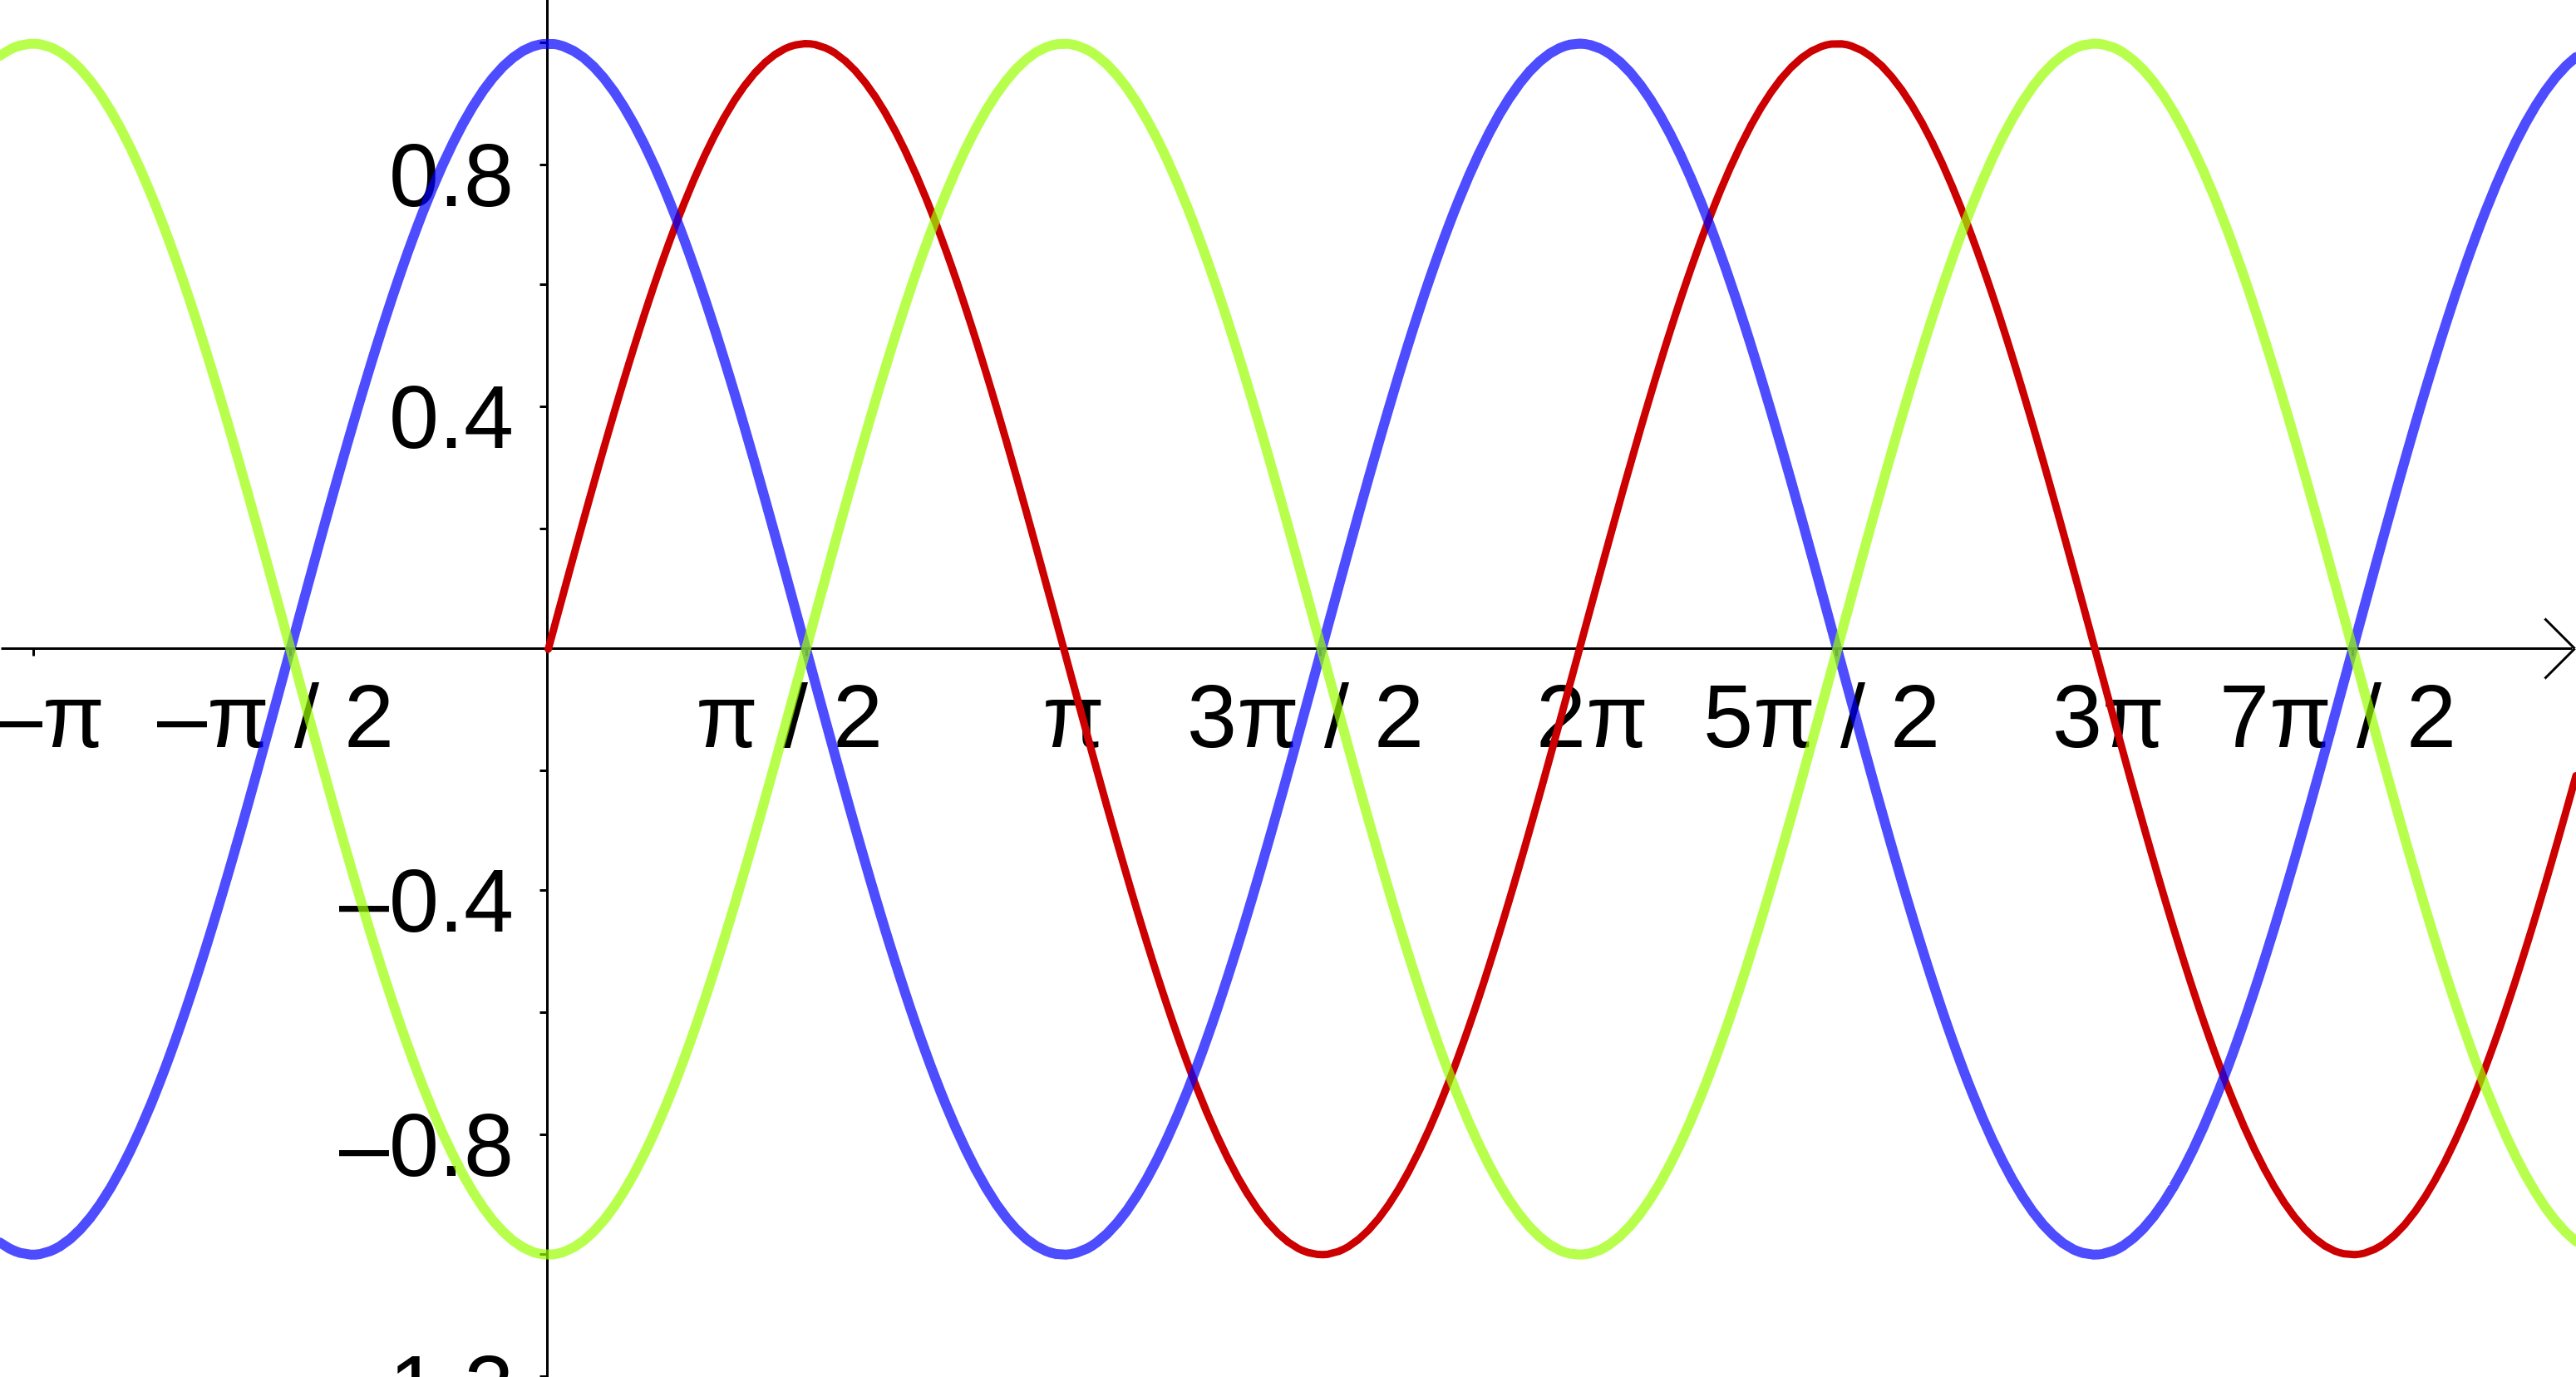
\includegraphics[scale=0.14]{images/ejemplos_senos}
  \caption{Ondas desfasadas}
  \label{fig:ejemplos_senos}
\end{figure}

\section{Valores rms}
El \textbf{valor RMS} o \textbf{valor eficaz}, es el valor de tensión o corriente alterna que produce la misma potencia que su equivalente en corriente continua.

No debe confundirse el valor eficaz con el \textbf{valor promedio}. El valor promedio de una tensión es la suma algebraica de las áreas respecto de la longitud de la curva. Si se analiza la corriente alterna senoidal, se observará que el valor promedio de tensión es de $0\; V$. No ocurre lo mismo con la \textbf{tensión eficaz}.

\begin{figure}[htbp]
  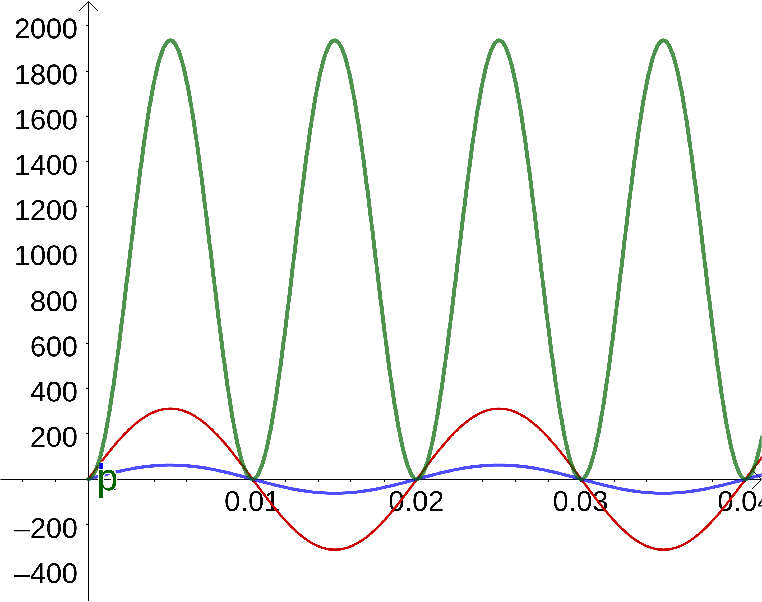
\includegraphics[scale=0.14]{images/potencia_alterna}
  \caption{Entrega de potencia en una corriente alterna senoidal}
  \label{fig:potencia_alterna}
\end{figure}

Al analizar la figura \ref{fig:potencia_alterna}, se puede observar tres ondas senoidales en fase. La más pequeña (azul), corresponde a la corriente eléctrica, medida en Amperes. La onda intermedia es la tensión (roja), expresada en Voltios. Estas ondas, poseen un semiciclo positivo y un semiciclo negativo, lo que indica un cambio en el sentido de la corriente.

La onda que toma mayor amplitud (verde), es la \textbf{potencia entregada}, calculada como el producto entre la tensión y la corriente eléctrica. Como se puede observar, todo el tiempo es positiva (excepto en los instantes 0, 0,1s y 0,2s).

Entonces, el problema de hallar la tensión eficaz, reside en observar para qué valor de tensión continua, la potencia entregada sería la misma que la de la onda más grande (verde) de la figura \ref{fig:potencia_alterna}.

A continuación se supondrá que se aplica una tensión con valor de pico $Vp$ y corriente de pico $Ip$ sobre una resistencia $R$.

\begin{eqnarray*}
	p(t)= i(t)^{2} R \\
	p(t)= [Ip sen(\omega t)]^{2} R \\
	p(t)= Ip^{2}sen^{2}(\omega t)R \\
\end{eqnarray*}
En este punto se utiliza la identidad trigonométrica $sen^{2}(\omega t) = \frac{1}{2}(1-cos(2\omega t))$.
\begin{eqnarray*}
	p(t)= Ip^{2}[\frac{1}{2}(1-cos(2 \omega t))]R \\
	p(t)=\frac{Ip^{2}R}{2}-\frac{Ip^{2}R}{2}cos(2 \omega t)
\end{eqnarray*}
Se anula el segundo término  por poseer valor medio igual a 0
 $$	p(t)=\frac{Ip^{2}R}{2} $$

Como se desea evaluar el valor de corriente continua equivalente, se supondrá que ahora se aplicó una corriente directa $I_{DC}$ a la misma carga resistiva. Su potencia $P_{DC}$ se calcularía de la siguiente forma:

$$ P_{DC} = I_{DC}^{2}R $$

Al igualar $P_{DC}$ con $p(t)$, se obtiene:
\begin{eqnarray*}
	p(t)=P_{DC} \\
	\frac{Ip^{2}R}{2}=I_{DC}^{2}R \\
	I_{DC}=\frac{Ip}{\sqrt{2}}=0,707Ip
\end{eqnarray*}

Es decir, que el valor de corriente continua equivalente de una corriente senoidal alterna es 0,707 su valor de pico. Este mismo análisis puede realizarse con la tensión, obteniendo el mismo valor.

Mediante el cálculo se puede demostrar a través de la integración, pero excede los temas de este curso.

\begin{conclusiones}
	Las siguientes ecuaciones permiten hallar valores eficaces a partir de valores de pico.
	\begin{equation}
		I_{RMS} = \frac{1}{\sqrt{2}}I_{PICO}=I_{PICO}\times 0,707
	\end{equation}
	\begin{equation}
		V_{RMS} = \frac{1}{\sqrt{2}}V_{PICO}=V_{PICO}\times 0,707
	\end{equation}
	Las siguientes ecuaciones, despejadas de las anteriores, permiten encontrar valores de pico a partir de valores eficaces.
	\begin{equation}
		I_{PICO} = \sqrt{2}I_{RMS}=I_{RMS}\times 1,414
	\end{equation}
	\begin{equation}
		V_{PICO} = \sqrt{2}V_{RMS}=V_{RMS}\times 1,414
	\end{equation}
\end{conclusiones}

\section{Respuesta de resistores, capacitores e inductores a la corriente alterna}
\subsection{Régimen transitorio}
Los cambios en los circuitos en las redes que poseen inductancia y capacidad no son instantáneos. Por ello, es conveniente evaluar el \textbf{régimen transitorio} de los circuitos, que corresponde a la respuesta que se produce ante una variación en el circuito hasta que se alcanza el \textbf{régimen permanente}, que es el momento en el cual los valores permanecen estables.
En el caso de una red capacitiva, los transitorios son:
\begin{itemize}
	\item Fase de carga.
	\item Fase de descarga.
\end{itemize}
En una red inductiva, los transitorios son:
\begin{itemize}
	\item Fase de almacenamiento.
	\item Fase de liberación.
\end{itemize}
\subsubsection{Fase de carga de una red capacitiva}
Al conectar un capacitor $C$ a una fuente de alimentación $V$ (por el momento, se supondrá que es continua) en serie con una resistencia $R$, éste acumula carga entre sus placas. Al principio, el movimiento de cargas es muy veloz, pero transcurrido un tiempo, el incremento es mucho más lento, hasta que finalmente se estabiliza. Esto se modela con la ecuación:
\begin{equation}
	\label{eq:carga_capacitor_i}
	i(t)=\frac{V}{R}e^{-t / \tau}
\end{equation}
Donde $\tau = RC $ se denomina \textbf{constante de tiempo} y se mide en segundos.

Para deducir que $\tau$ refiere a tiempo, se utilizará la Ley de Ohm, la ecuación \ref{eq:capacitancia} y la ecuación \ref{eq:2}: $$ \tau = RC = (V/I)(Q/V)=(\frac{V}{Q/t})(Q/V)=t$$

Por el contrario, la tensión en el capacitor será mínima en el instante en el cual se suministra tensión entre las placas, e irá aumentando a medida que las placas se vayan cargando. Cuando esto ocurra, la tensión será la de la fuente. Esto se modela con la ecuación:
\begin{equation}
	\label{eq:carga_capacitor_v}
	v(t)=V(1-e^{-t / \tau})
\end{equation}

Como una buena aproximación, se sabe que luego de cinco constantes de tiempo, la carga del capacitor es casi completa (más el 90\%). Esto suele ser útil para realizar cálculos y estimaciones.

Para demostrarlo, se reemplaza $t=5\tau$ en la ecuación \ref{eq:carga_capacitor_v}, obteniendo:

\begin{eqnarray*}
	v(5\tau)=V(1-e^{-5\tau / \tau} \\
	v(5\tau)=V(1-e^{-5} \\
	v(5\tau)=V-Ve^{-5} \\
	v(5\tau)=V-0,07358V  \\
	v(5\tau)=0,926V
\end{eqnarray*}

Lo que ocurre con la corriente en este periodo de tiempo es que se vuelve muy cercana a $0 A$, debido a que las placas están casi cargadas por completo. El razonamiento es el mismo, pero reemplazando $t=5\tau$ en la ecuación \ref{eq:carga_capacitor_i}, y se dejará para ejercicio del lector.

\begin{conclusiones}
	La tensión de un capacitor no varía de forma instantánea.
		
	Durante la fase de carga, la corriente comienza siendo muy alta, pero luego de cinco constantes de tiempo, se vuelve cercana a $0\; A$. Por el contrario, la tensión comienza siendo $0\; V$ y transcurridos cinco constantes de tiempo, se vuelve cercana al valor de la fuente de alimentación.
	
	El mayor cambio de voltaje y de corriente ocurren durante la primera constante de tiempo.
	
	Cuando el transitorio comienza, el circuito equivalente del capacitor es un cortocircuito, pero cuando el transitorio finalizó, el circuito equivalente del capacitor es un circuito abierto.
\end{conclusiones}
\subsubsection{Fase de descarga de una red capacitiva}
La manera más rápida de descargar un capacitor es cortocircuitando sus contactos. Esto hará que la corriente fluya de una placa a la otra de forma acelerada, pero esto conlleva varios riesgos para el operario y para el componente, que, como mínimo, provocará un chispazo, dependiendo de su capacidad.

Si se piensa en el circuito utilizado para la fase de carga (batería en serie con resitencia y capacitor), cortocircuitando la batería (o reemplazándola por un cable), el capacitor se descargará por la resistencia de forma más lenta y segura, pero es importante notar que la polaridad de la corriente se invertirá. La curva de descarga de la tensión será similar a la curva de carga de la corriente:
\begin{equation}
	\label{eq:descarga_capacitor_v}
	v(t)=Ve^{-t / \tau}
\end{equation}
Y la corriente será la misma que en la fase de carga, pero con la polaridad invertida:
\begin{equation}
	\label{eq:descarga_capacitor_i}
	i(t)=-\frac{V}{R}e^{-t / \tau}
\end{equation}
Al igual que en la fase de carga, se supone que la fase de descarga estará casi completa luego de cinco constantes de tiempo.

En este análisis de respuesta transitoria, se omitirán las condiciones iniciales. Esto quiere decir, que se supondrá que los capacitores \textbf{siempre están descargados}.

\subsubsection{Fase de almacenamiento en una red inductiva}

Existen semejanzas entre la \textbf{tensión de una bobina} y la \textbf{corriente de un capacitor}. Para el siguiente análisis, se supondrá un circuito RL serie (fuente de tensión continua, interruptor, resistencia e inductor).

Así como un capacitor almacena energía en forma de campo eléctrico entre sus placas, una bobina almacena energía en forma de campo magnético. En el instante en el que se cierra el interruptor, la bobina ofrece una \textbf{acción de bloqueo}, efecto de la \textit{Ley de Lenz} (refiérase al capítulo correspondiente a \textit{Máquinas eléctricas} para un mejor desarrollo). Esta acción de bloqueo, impedirá la aparición de corriente de manera instantánea, provocando una curva de respuesta de corriente muy similar a la de tensión del capacitor: al principio $i_L = 0$, luego se incrementará rápidamente, y finalmente se acercará con menor rapidez al valor determinado por la red $V/R$. Este comportamiento es modelado con la siguiente ecuación:


\begin{equation}
	\label{eq:almacenamiento_inductor_i}
	i(t)=\frac{V}{R}(1-e^{-t / \tau})
\end{equation}

Con la constante de tiempo, esta vez definida como $\tau = \frac{L}{R} $, extendiéndose el análisis sobre la misma realizada con los capacitores.

La tensión en la bobina será:
\begin{equation}
	\label{eq:almacenamiento_inductor_v}
	v(t)=Ve^{-t / \tau}
\end{equation}

\begin{conclusiones}
	La fase de almacenamiento finaliza aproximadamente en cinco constantes de tiempo.
	
	En una red inductiva, el cambio de corriente nunca es instantáneo, debido a sus características de bloqueo.
	
	Apenas se cierra el interruptor, la bobina se convierte en un circuito abierto, pero luego de que finalice su fase de almacenamiento, se comporta como un cortocircuito.
\end{conclusiones}

\subsubsection{Fase de liberación en una red inductiva}

En una red capacitiva, la energía se mantenía almacenada en forma de campo eléctrico, aún cuando se desconectara la fuente de tensión, debido a la atracción de cargas entre las placas (sólo se descargaría por las corrientes de fuga). En un inductor, al eliminar el flujo de corriente eléctrica, el campo magnético se liberará rápidamente, y la reducción abrupta de corriente provocará un chispazo en los contactos. Como la tensión es producto de la \textbf{variación en la corriente}, y la variación es abrupta, la tensión será muy alta.

Al liberar la energía, el inductor sigue la curva de descarga de las siguientes ecuaciones de tensión y corriente respecto del tiempo:
\begin{equation}
	\label{eq:liberacion_inductor_v}
	v(t)=-Ve^{-t / \tau}
\end{equation}
\begin{equation}
	\label{eq:liberacion_inductor_v}
	i(t)=\frac{V}{R} e^{-t / \tau}
\end{equation}

\begin{conclusiones}
	Los inductores y capacitores, idealmente, no disipan energía, sino que la almacenan como campo eléctrico (en el caso del capacitor) o como campo magnético (en el caso del inductor).
	
	Todas las fases transitorias analizadas tienen una duración aproximada de cinco constantes de tiempo.
\end{conclusiones}

\subsection{Respuesta del resistor}

Para frecuencias de línea ($50\; Hz$ en el caso de Argentina), las cargas resistivas tienen un comportamiento lineal, y por ello puede aplicarse directamente la Ley de Ohm para calcular sus tensiones y corrientes.

\begin{figure}[htbp]
%  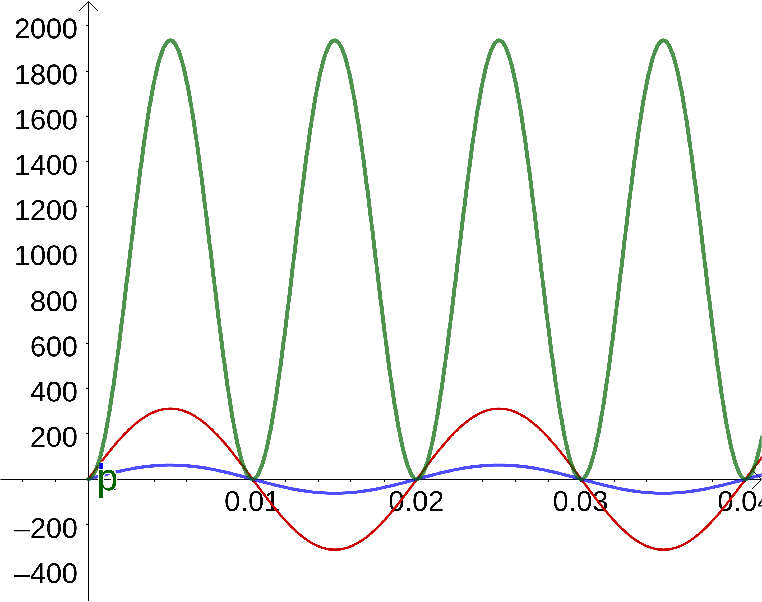
\includegraphics[scale=0.14]{images/potencia_alterna}
  \caption{Curvas de respuesta del resistor en corriente alterna}
  \label{fig:respuesta_resistor_curvas}
\end{figure}
\begin{figure}[htbp]
%  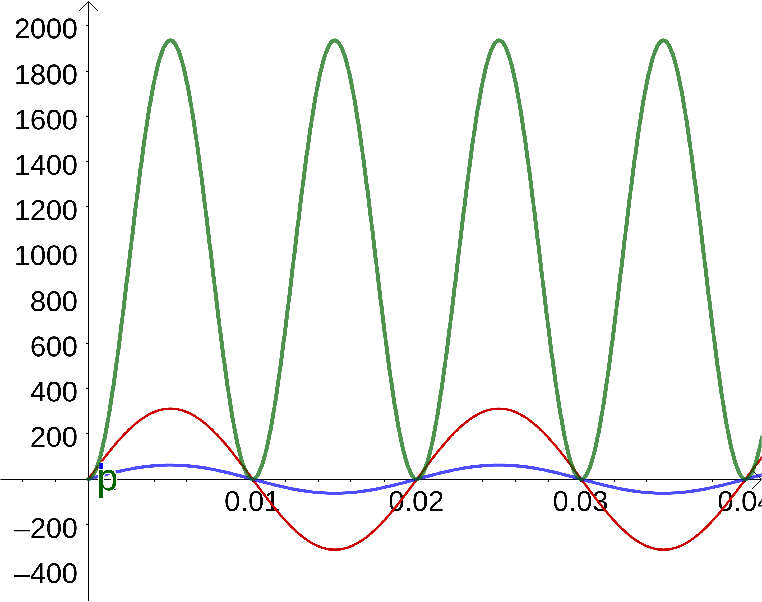
\includegraphics[scale=0.14]{images/potencia_alterna}
  \caption{Circuito resistivo con una fuente de corriente alterna}
  \label{fig:respuesta_resistor_circuito}
\end{figure}

$$ i = \frac{V_{RMS} \times sen(\omega t)}{R} = \frac{V_{RMS}}{R} sen(\omega t) = I_{RMS} sen(\omega t) $$

Como se observa en la figura~\ref{fig:respuesta_resistor_curvas}, la fase de la corriente y la tensión es la misma. Por lo tanto, la variación de corriente y tensión ocurren en la misma proporción y puede considerarse:

\begin{equation}
	\label{eq:i_resistor_alterna}
	I_{RMS} = \frac{V_{RMS}}{R}
\end{equation}
\begin{equation}
	\label{eq:i_resistor_alterna}
	V_{RMS} = I_{RMS}\times R
\end{equation}

\subsection{Respuesta del inductor}

La tensión a través de un inductor está directamente relacionado con la velocidad de cambio de la corriente a través del mismo. En corriente alterna, esta variación está dada, entre otros factores, por la frecuencia de la red. Por ello, existe una relación entre la frecuencia, la tensión en el inductor y su valor de inductancia.

\begin{eqnarray*}
	v_L = L \frac{di_L}{dt} \\
	v_L = L \frac{d}{dt}(Ip\times sen(\omega t)) \\
	v_L = L( \omega Ip\times cos (\omega t)) \\
	v_L = \omega L Ip\times cos(\omega t) \\
	v_L = \omega L Ip\times sen(\omega t +90^{\circ}) \\
\end{eqnarray*}

Como se explicó antes, el valor de pico está relacionado con $\omega=2\pi f$, y por $L$ como se explicó anteriormente. También puede apreciarse que la corriente y la tensión difieren en su fase por 90º.

\begin{conclusiones}
	En el inductor, la tensión $v_L$ va por delante 90º a la corriente $i_L$. 
	\begin{equation}
		\label{eq:i_inductor}
		i_L = Ip\times sen(\omega t)
	\end{equation}
	
	\begin{equation}
		\label{eq:v_inductor}
		v_L = \omega \times L \times Ip \times sen(\omega t + 90^{\circ})
	\end{equation}
	
\end{conclusiones}

\subsection{Respuesta del capacitor}

La tensión en un capacitor está limitada por la velocidad a la cual se depositan o liberan las cargas entre sus placas, y por ello, a mayor frecuencia, mayor corriente.

Por otra parte, mientras mayor sea el valor de capacitancia, mayor será la corriente capacitiva resultante, debido a que $i = C(dv/dt)$.

\begin{eqnarray*}
	i_C = C \frac{dv_C}{dt} \\
	i_C = C \frac{d}{dt}(Vp\times sen(\omega t)) \\
	i_C = C (\omega \times Vp \times cos(\omega t)) \\
	i_C = \omega \times C \times Vp \times sen(\omega t + 90^{\circ}) \\
\end{eqnarray*}

\begin{conclusiones}
	En el capacitor, la corriente $i_C$ va por delante a la tensión $v_C$ unos 90º. 
	\begin{equation}
		\label{eq:v_capacitor}
		v_C = Vp\times sen(\omega t)
	\end{equation}
	\begin{equation}
		\label{eq:i_capacitor}
		i_C = \omega \times C \times Vp \times sen(\omega t + 90^{\circ})
	\end{equation}
\end{conclusiones}

\subsection{Impedancia}

La \textbf{oposición} en un circuito de corriente alterna, está dada por la Ley de Ohm. Ocurre que, al incorporar capacitancias e inductancias, la idea de \textbf{resistencia} resulta insuficiente para modelar la oposición.

Si se vuelve a analizar lo expuesto en este capítulo según la relación $\text{Efecto} = \frac{\text{Causa}}{\text{Oposición}} \rightarrow \text{Oposición} = \frac{\text{Causa}}{\text{Efecto}}$, como se ha hecho anteriormente, y volviendo a suponer a la corriente como el \textbf{efecto} que produce la \textbf{tensión}, se puede abordar la idea de \textbf{impedancia}, definida como \textit{la oposición que presenta un circuito de de corriente alterna al aplicarle una tensión}.

\begin{equation}
	\label{eq:impedancia}
	Z=\frac{V}{I}
\end{equation}

En la ecuación \ref{eq:impedancia}, $Z$ refiere a la impedancia, y tanto $V$ como $I$ son fasores (números complejos que representan a la tensión y corriente alterna respectivamente).

La impedancia, cuyo término proviene de la idea de \textit{impedir el paso de la corriente}, estará compuesta por una parte \textbf{resistiva}, y una parte \textbf{reactiva} (que \textit{reacciona}, o no sólo consume energía sino que también puede almacenarla y devolverla eventualmente). Los componentes \textbf{reactivos} serán los inductores y los capacitores.

Para el caso del inductor, según las ecuaciones \ref{eq:i_inductor} y \ref{eq:v_inductor}, se define a la oposición del mismo como \textbf{reactancia inductiva $X_L$} de la siguiente forma:

$$ X_L = \frac{\omega \times L \times Ip \times sen(\omega t)}{Ip\times sen(\omega t)} = \omega L $$

De manera análoga, para el capacitor y según las ecuaciones \ref{eq:i_capacitor} y \ref{eq:v_capacitor}, se define como \textbf{reactancia capacitiva $X_C$} a:

$$ X_C = \frac{Vp\times sen(\omega t)}{\omega \times C \times Vp \times sen(\omega t)} = \frac{1}{\omega C} $$

La \textbf{impedancia Z}, puede ser definida como un fasor que relaciona la \textbf{resistencia} con la \textbf{reactancia} de la siguiente forma:

\begin{equation}
	\label{eq:impedancia_rectangular}
	Z = R + j(X_L-X_C)
\end{equation}

\section{Fasores}
Los fasores permiten relacionar tensiones y corrientes alternas senoidales de una forma más sencilla que si se trabajara directamente con las ondas.

Como ya se sabe, una onda senoidal se define completamente por su \textbf{amplitud}, \textbf{frecuencia} y \textbf{fase}. Como se trabajará siempre con la misma frecuencia, sólo se necesitará la amplitud y la fase para poder definirlas, y ésto se puede hacer a través de vectores, que se llamarán fasores.

%Un \textbf{fasor} es un número complejo que tiene como variable a su argumento.
%$$ U = | U | e^{j\omega t} $$
%Aplicando la fórmula de Euler en la expresión anterior, resulta,
%$$ U = | U | cos (\omega t) + j|U| sen(\omega t) $$

Un \textbf{fasor} es un vector giratorio que permite representar una onda de corriente o de tensión. El módulo del vector representa el valor eficaz de la onda, mientras que la frecuencia será la velocidad a la que giran (cuestión que será omitida, porque se supone que todos giran a la misma velocidad angular), y la fase está representada por el ángulo entre fasores.

En otras palabras, los fasores representan una fotografía instantánea de la posición del vector giratorio que define las ondas de tensión y de corriente.

La impedancia, también es un número complejo y fasor, definido como $Z= R+j(X_L - X_C)$, y $X_L = \omega L $, $X_C = \frac{1}{\omega C}$, como se ha visto anteriormente. La diferencia con los fasores de tensión y de corriente, es que la impedancia no se encuentra girando sino que está estática.

Para realizar operaciones con fasores (lo cual es más sencillo que operar con ecuaciones de ondas), se debe utilizar el álgebra de los números complejos, resultando más conveniente utilizar la \textbf{forma rectangular} para realizar sumas y restas, y la \textbf{forma polar} para realizar multiplicaciones y divisiones.

\section{Potencia}

La ecuación general de la potencia es: $$ p = vi $$

Nótese que las tres magnitudes varían en el tiempo (y por ello están escritas en minúscula). Para el caso de corriente continua, bastaría con operar utilizando la ecuación  \ref{eq:pot}, pero cuando se trata de una corriente alterna senoidal, este cálculo es algo más complejo, y más aún cuando existen desfasajes entre la tensión y la corriente aplicada a la carga.

En corriente alterna se definen tres tipos de potencia: la activa, reactiva y aparente, y a su vez, se introduce un factor de potencia.

La \textbf{potencia activa} es la que consume cualquier aparato eléctrico para funcionar, y se mide en Watts ($W$).

En corriente alterna las bobinas y los condensadores no sólo consumen energía, sino que también la acumulan. Entonces, una cierta cantidad de potencia se mueve dentro del circuito pero no sale de él, y recibe el nombre de \textbf{potencia reactiva}. Éste tipo de potencia se mide en Volt-Amperes reactivos ($VAr$).

En el caso de la potencia reactiva, no hay un real consumo de energía, ya que primero se consume y luego se devuelve, pero este fenómeno implica que el proveedor de energía deba entregar toda esta potencia (la activa y también la reactiva, aunque luego ésta última vaya a ser devuelta), con su consecuente necesidad de dimensionar los conductores para un consumo mayor. Pareciera ser que, como la potencia reactiva no es disipada, entonces no  debería ser tenida en cuenta, pero para el proveedor de energía es importante, ya que debe entregarla de todos modos, aunque luego sea devuelta. Desde el punto de vista del consumidor, una parte de la energía se pide ``prestada" para hacer funcionar elementos con consumos reactivos (como motores o transformadores) y luego se devuelve a la red, pero de todos modos, aunque esta energía no haya sido parte de la energía aprovechada por los elementos de la red, fue necesaria para hacerlos funcionar correctamente.

La \textbf{potencia aparente} corresponde a la energía que se entrega por el proveedor, que no sólo expresa el valor de potencia activa sino también a la potencia reactiva. Esto llevaría a pensar que la potencia aparente es simplemente la suma de ambas potencias, pero debe recordarse que en corriente alterna, ambos valores corresponden a ondas, y por lo tanto su cálculo no es tan simple de realizar. La unidad que se utiliza para medir la potencia aparente es el Volt-Ampere ($VA$).

A continuación, se muestran imágenes para distintos tipos de consumo.
\begin{itemize}
	\item Para el consumo resistivo puro de la figura \ref{fig:potencia_alterna_resistiva}, las ondas de corriente y de tensión están en fase. La potencia será el producto entre ambas, y como se observa en la gráfica, siempre es positiva (está por arriba del eje de abscisas). Esto significa que siempre se está entregando potencia activa.
	\item En los consumos capacitivo puro e inductivo puro de las figuras \ref{fig:potencia_alterna_capacitiva} y \ref{fig:potencia_alterna_inductiva} respectivamente, puede apreciarse que durante medio ciclo de potencia, el sistema entrega potencia, pero la otra mitad de tiempo la absorbe. En otras palabras, la potencia activa es de $0\; W$, porque nunca se está disipando energía, y la potencia es puramente reactiva.
	\item En las curvas de la figura \ref{fig:potencia_alterna_mixta}, se observa un consumo real, que es en parte reactivo y en parte activo, pero la parte activa es mayor que la reactiva. Es decir, que la potencia entregada es mayor a la potencia devuelta. Esto es lo que ocurre en las redes eléctricas reales.
\end{itemize}
% Imágenes de consumo resistivo, inductivo, capacitivo y mixto.
\begin{figure}[htbp]
  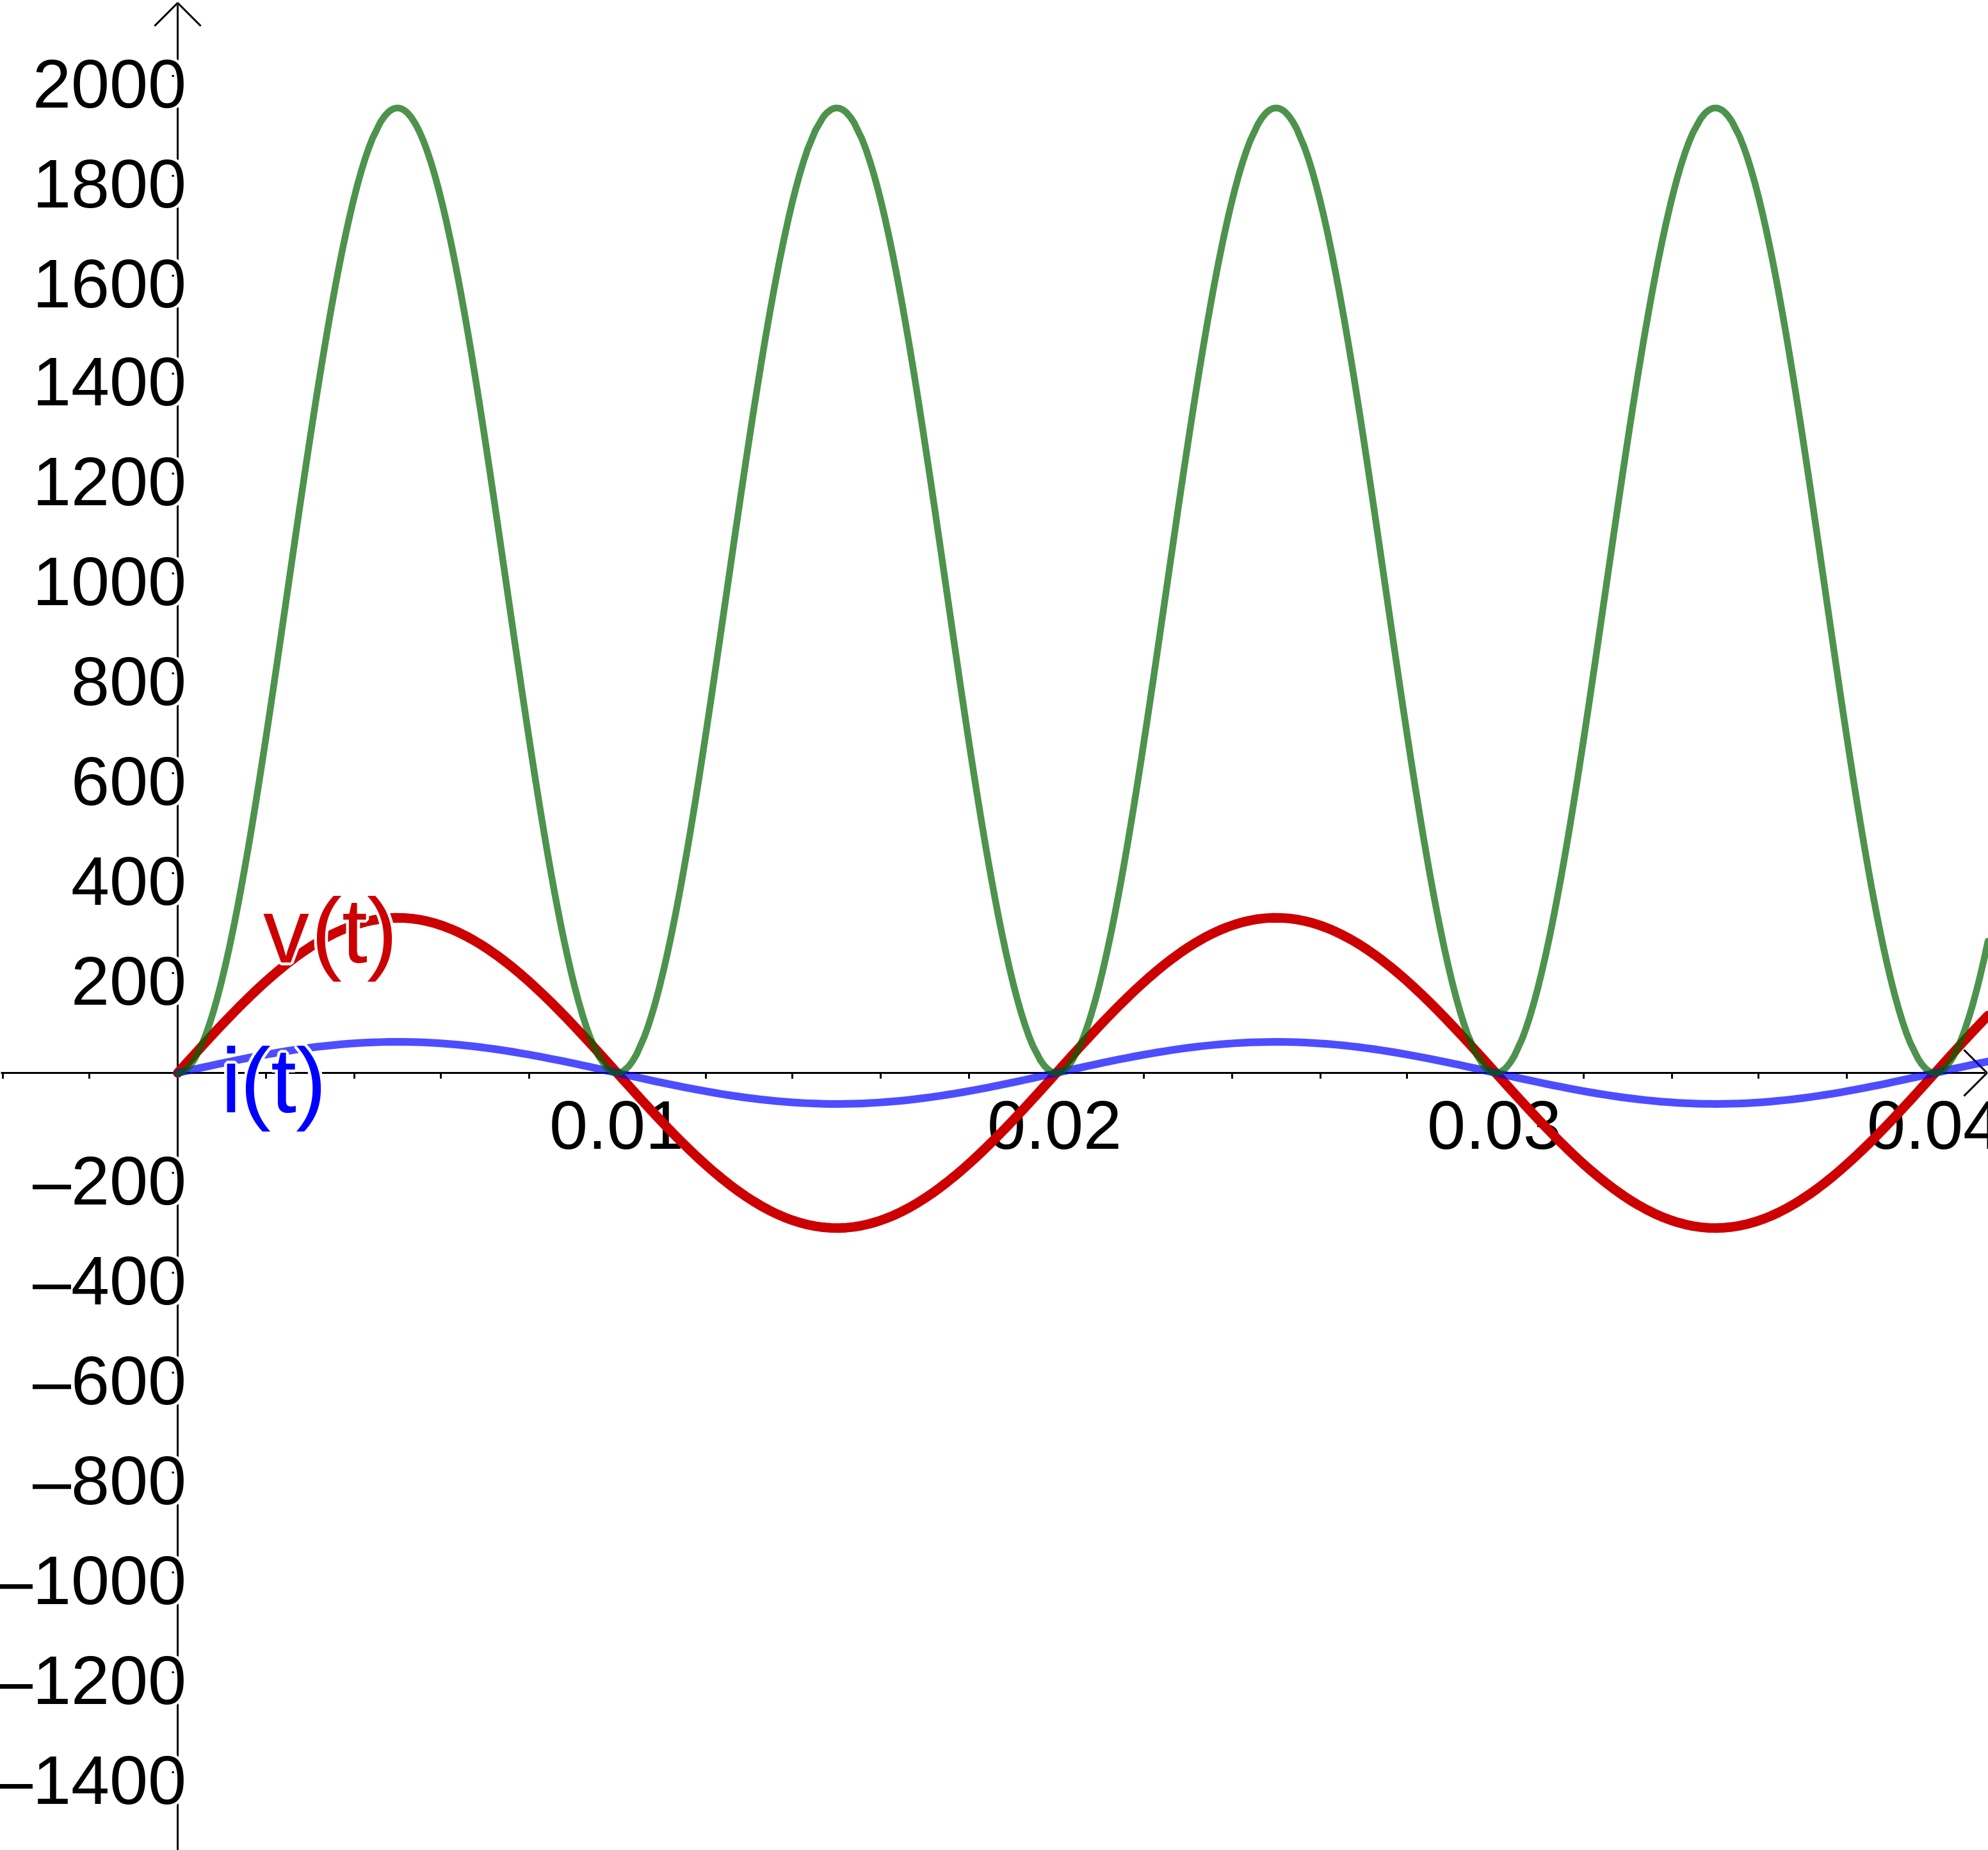
\includegraphics[scale=0.1]{images/potencia_alterna_resistiva}
  \caption{Respuesta de un circuito resistivo puro en C.A.: corriente en azul, tensión en rojo y potencia en verde}
  \label{fig:potencia_alterna_resistiva}
\end{figure}

\begin{figure}[htbp]
  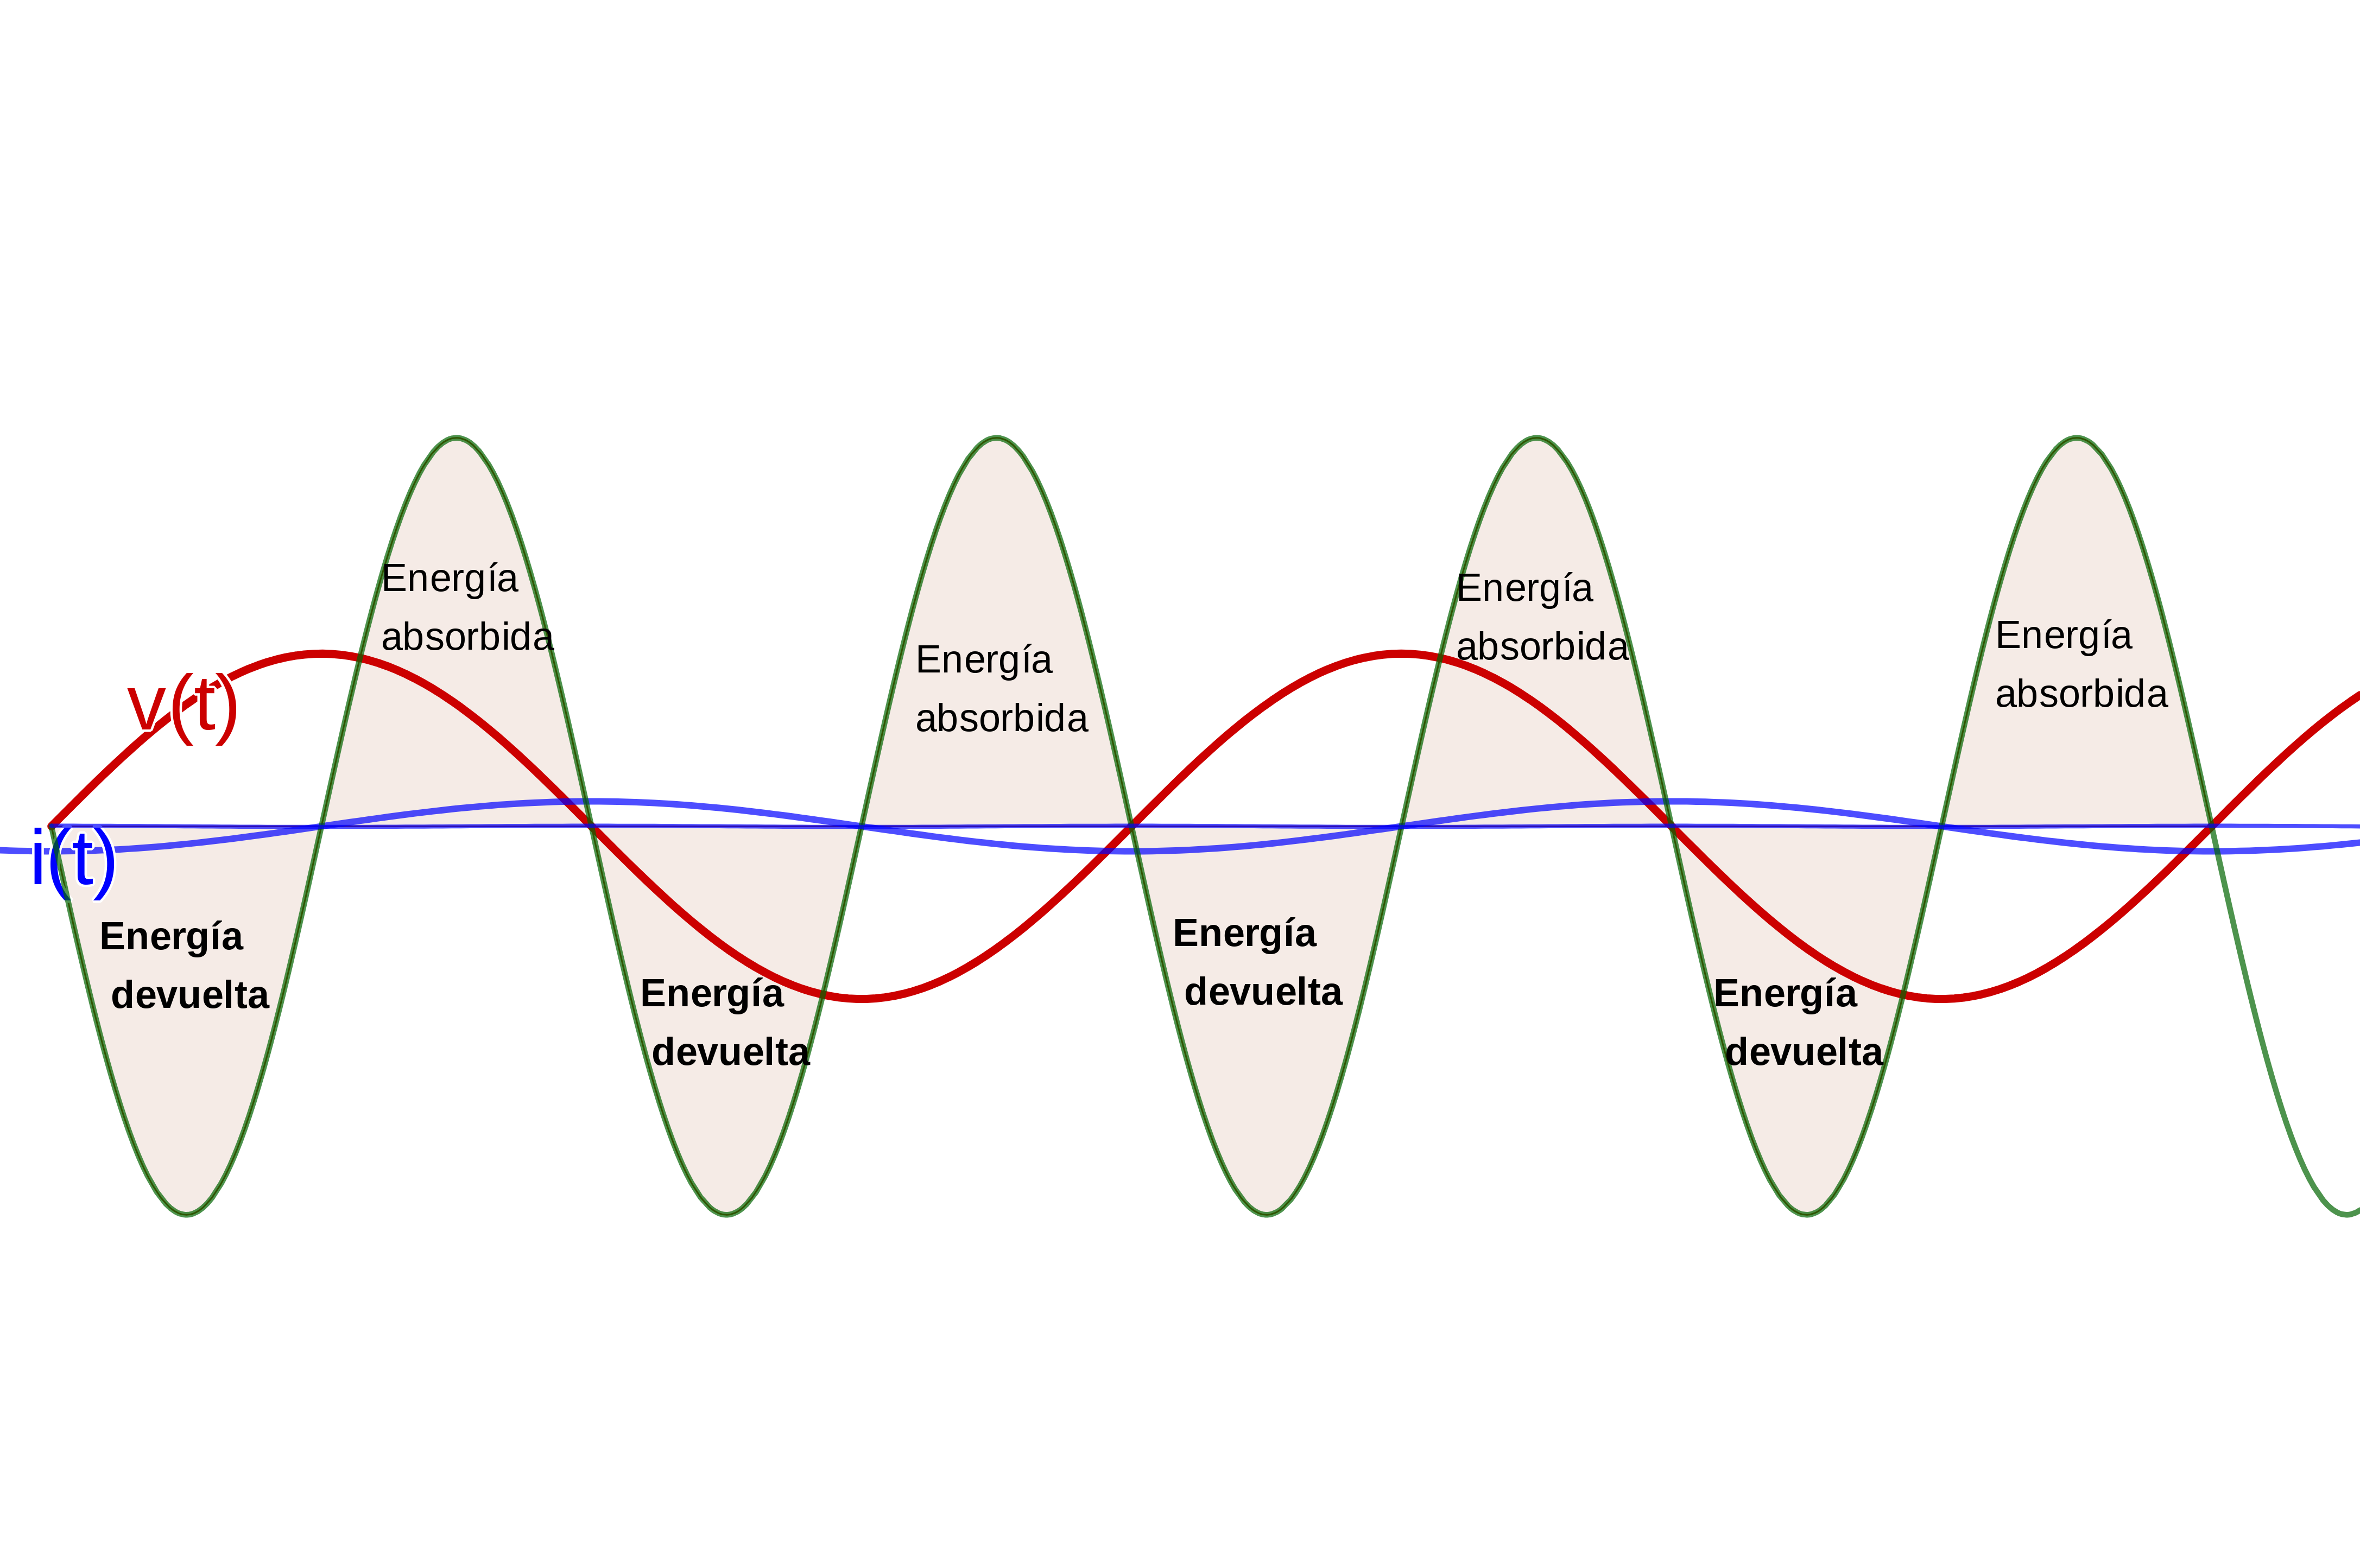
\includegraphics[scale=0.1]{images/potencia_alterna_inductiva}
  \caption{Respuesta de un circuito inductivo puro en C.A.: corriente en azul, tensión en rojo y potencia en verde}
  \label{fig:potencia_alterna_inductiva}
\end{figure}

\begin{figure}[htbp]
  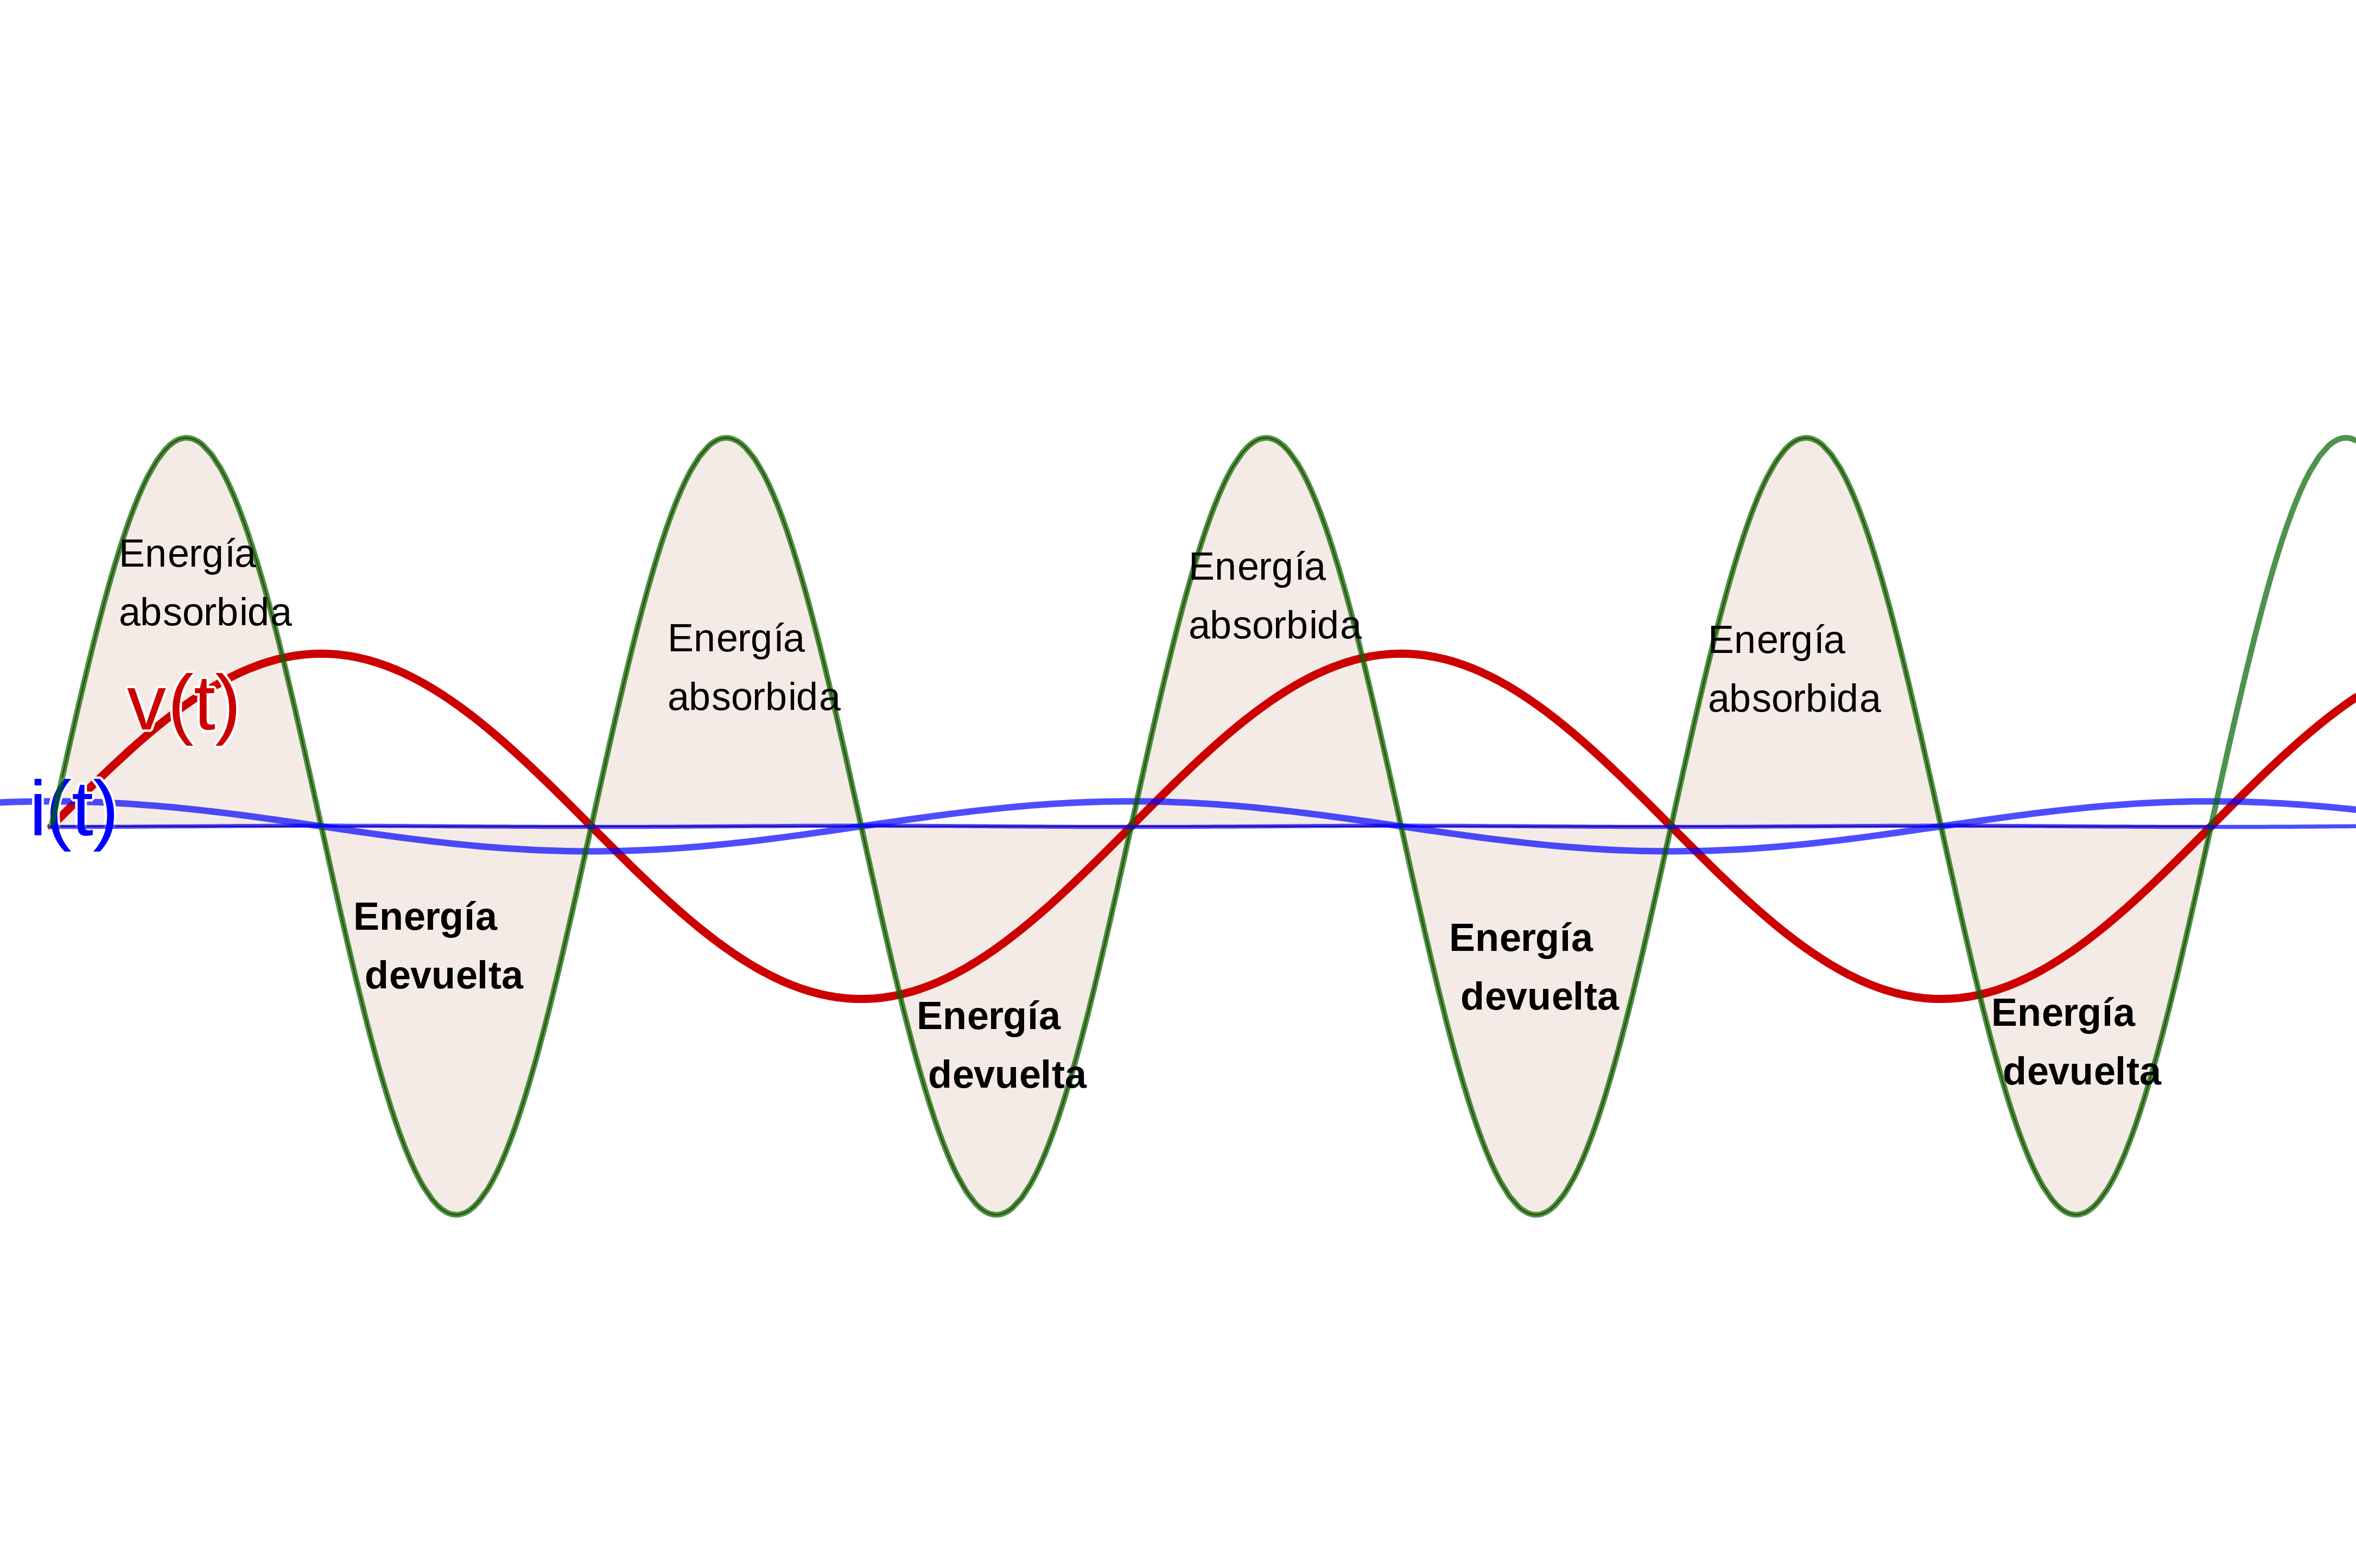
\includegraphics[scale=0.1]{images/potencia_alterna_capacitiva}
  \caption{Respuesta de un circuito capacitivo puro en C.A.: corriente en azul, tensión en rojo y potencia en verde}
  \label{fig:potencia_alterna_capacitiva}
\end{figure}

\begin{figure}[htbp]
  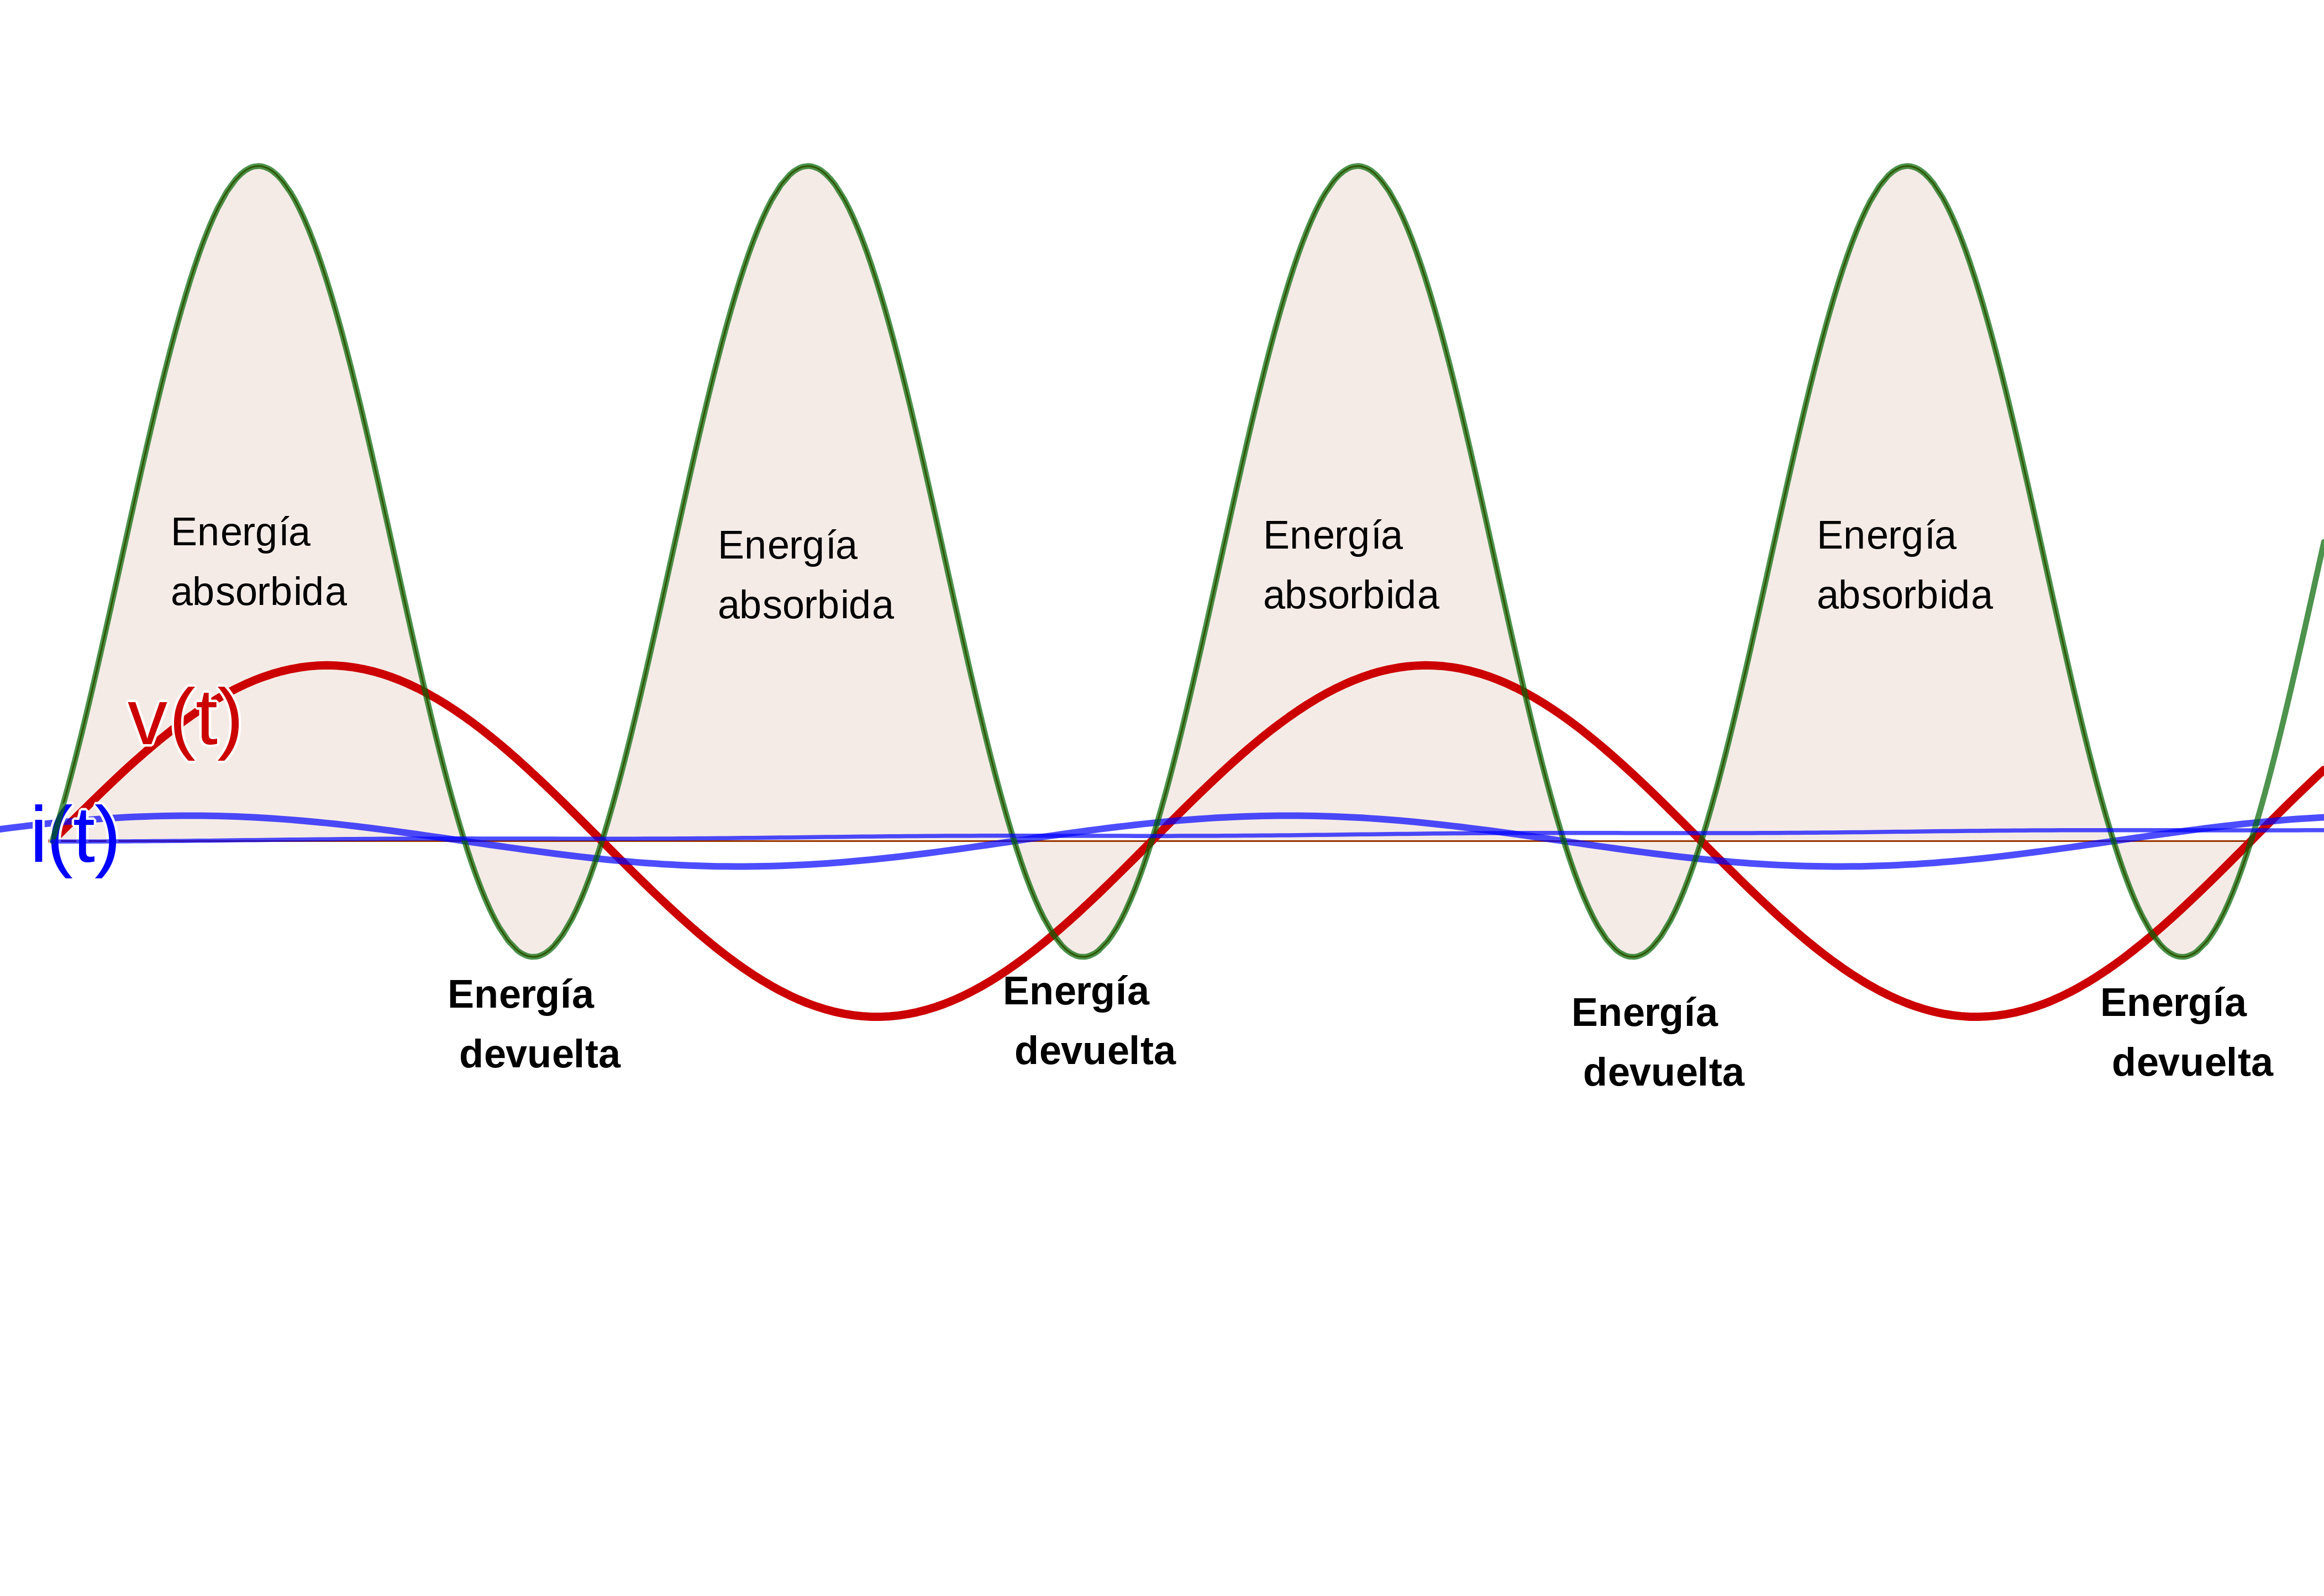
\includegraphics[scale=0.1]{images/potencia_alterna_mixta}
  \caption{Respuesta de un circuito real (resistivo y reactivo) en C.A.: corriente en azul, tensión en rojo y potencia en verde}
  \label{fig:potencia_alterna_mixta}
\end{figure}
Como la realización de operaciones con ecuaciones de ondas es algo complejo e impreciso, se verá a continuación cómo hacerlo con fasores.

\subsection{Triángulo de potencias}

Si se recuerda la representación fasorial de la impedancia, se verá que en el eje de ordenadas se expresaban los fasores de reactancia: hacia arriba $X_L$, y hacia abajo $X_C$, y en el eje de abscisas, el valor de resistencia $R$.

\begin{figure}[htbp]
  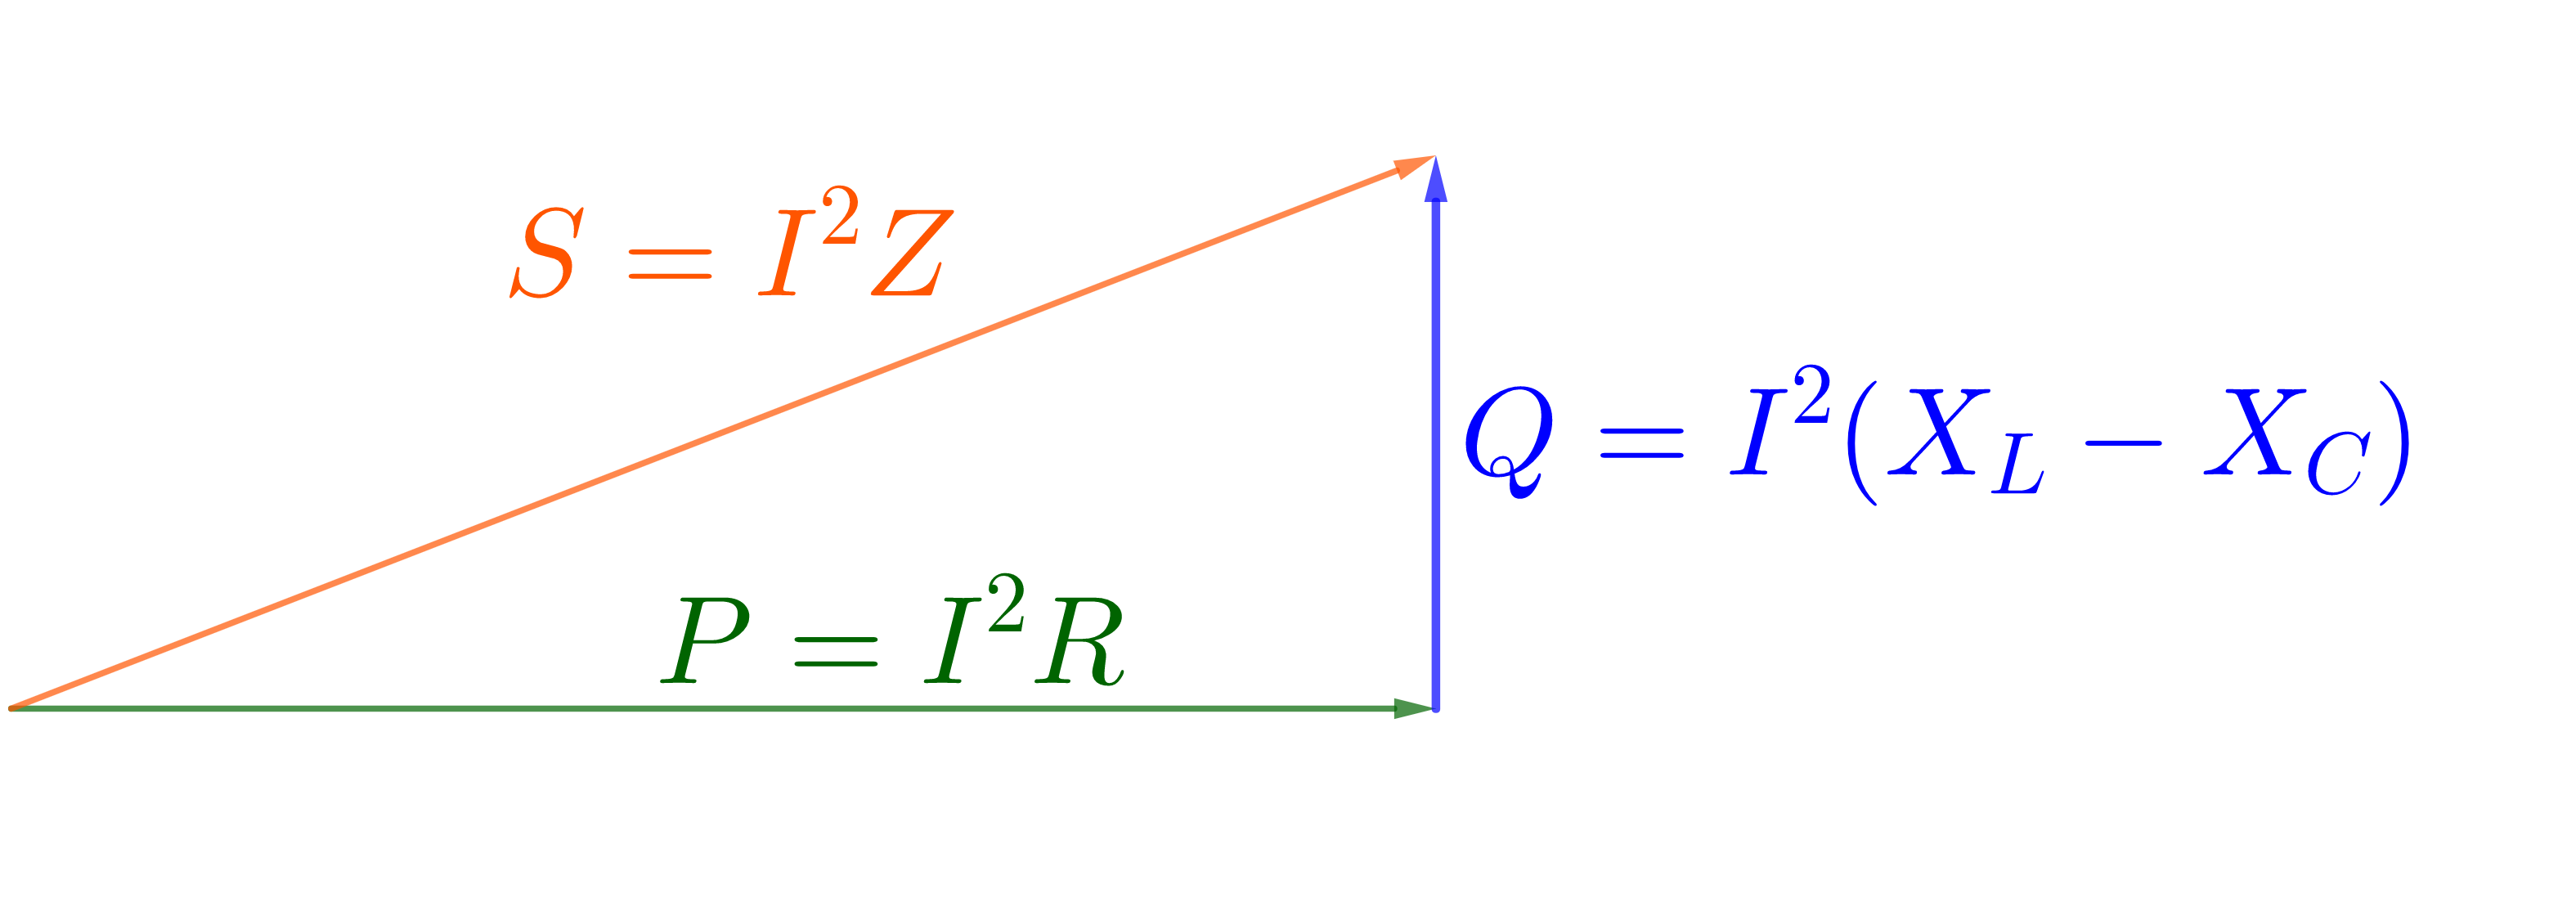
\includegraphics[scale=0.16]{images/triangulo_potencias}
  \caption{Triángulo de potencias}
  \label{fig:triangulo_potencias}
\end{figure}

El triángulo de potencias estará formado por:
\begin{itemize}
	\item La potencia activa $P$ en el eje de abscisas.
	\item La potencia reactiva $Q$ en el eje de ordenadas.
	\item La potencia aparente $S$ como la suma de ambos vectores.
	\item El ángulo entre $P$ y $S$, llamado $\varphi$.
\end{itemize}

De ese modo, la relación entre la potencia activa y la aparente es el \textbf{factor de potencia}, o también llamado \textbf{coseno de $\varphi$}, debido a que ésta es la forma en la cual se calcula.

Utilizando el Teorema de Pitágoras, se llega a la conclusión de que la relación entre las tres potencias es:

\begin{equation}
	\label{eq:potencias_alterna}
	S^{2}=P^{2}+Q^{2}
\end{equation}

Y dado que $S=V_{RMS}\times I_{RMS}$, utilizando trigonometría se pueden definir las potencias activa y reactiva como:

\begin{eqnarray}
	\label{eq:potencias_activa_reactiva}
	Q=V_{RMS}\times I_{RMS} \times sen(\varphi) \\
	S=V_{RMS}\times I_{RMS} \times cos(\varphi)
\end{eqnarray}

Como se indicó en el apartado anterior, la potencia reactiva implica el transporte de energía que no será aprovechada posteriormente. Las pérdidas en los cables por efecto Joule serán mayores aunque para el consumo efectivo de potencia activa no haya diferencias. Esto perjudica claramente a las empresas que suministran energía. Por este motivo, en talleres e industrias, se suele \textbf{penalizar el consumo reactivo excesivo}, limitando el \textbf{factor de potencia} a 0,8 (siendo 1 el valor ideal).

Por ello, suele ser necesario compensar la potencia reactiva con cargas capacitivas o inductivas.  